\documentclass[12pt, a4paper]{report}

% Essential Packages
\usepackage{float}
\usepackage[utf8]{inputenc}
\usepackage{graphicx}   % For handling the BITS logo and placeholders
\usepackage{geometry}   % For page margins
\usepackage{setspace}   % For line spacing
\usepackage{titlesec}   % For title formatting
\usepackage{times}      % Times New Roman font (standard for formal reports)
\usepackage{booktabs}   % REQUIRED for tables (\toprule, \midrule, \bottomrule)
\usepackage{amsmath}    % Standard math package for better equations
\usepackage{amsfonts}
\usepackage{amssymb}
\usepackage{listings}   % For formatting Python code blocks
\usepackage{xcolor}     % For coloring code blocks
\usepackage{subcaption}
\usepackage{siunitx}    % For physical units
\usepackage{multirow}   % For multi-row table cells
\usepackage{hyperref}
\usepackage{cleveref}
\usepackage{microtype}   % For \Cref cross-referencing

% Code Listing Style Configuration
\definecolor{codegreen}{rgb}{0,0.6,0}
\definecolor{codegray}{rgb}{0.5,0.5,0.5}
\definecolor{codepurple}{rgb}{0.58,0,0.82}
\definecolor{backcolour}{rgb}{0.95,0.95,0.92}

\lstdefinestyle{mystyle}{
    backgroundcolor=\color{backcolour},   
    commentstyle=\color{codegreen},
    keywordstyle=\color{magenta},
    numberstyle=\tiny\color{codegray},
    stringstyle=\color{codepurple},
    basicstyle=\ttfamily\footnotesize,
    breakatwhitespace=false,         
    breaklines=true,                 
    captionpos=b,                    
    keepspaces=true,                 
    numbers=left,                    
    numbersep=5pt,                  
    showspaces=false,                
    showstringspaces=false,
    showtabs=false,                  
    tabsize=2
}
\lstset{style=mystyle}

% Page Layout Settings
\geometry{
    top=1.0in,
    bottom=1.0in,
    left=1.25in, 
    right=1.0in
}
\onehalfspacing 

\begin{document}

%----------------------------------------------------------------------------------------
%    TITLE PAGE
%----------------------------------------------------------------------------------------
\begin{titlepage}
    \begin{center}
        \vspace*{0.5cm}
        
        {\Large A Project Report}\\[0.5cm]
        {\Large On}\\[0.5cm]
        
        {\Huge \bfseries Learning-Based Detection of Simulated Optical Injection-Locking Anomalies in Twin-Field Quantum Key Distribution}\\[0.5cm] 
        
        {\Large \textbf{BY}}\\[0.5cm]
        
        {\Large \textbf{MITHIL HARDIK ASTIK}}\\[0.2cm] 
        {\Large \textbf{2024B5A30923H}}\\[1cm]   
        
        {\Large Under the supervision of}\\[0.5cm]
        {\Large \textbf{Prof. T S L RADHIKA}}\\[0.5cm] 
        
        {\large SUBMITTED IN PARTIAL FULFILLMENT OF THE REQUIREMENTS OF}\\[0.3cm]
        {\Large \textbf{PHY F376: DESIGN PROJECT}}\\[1.5cm]
        
        % LOGO PLACEHOLDER
        \IfFileExists{BITS_LOGO.jpg}{\includegraphics[width=3cm]{BITS_LOGO.jpg}}{\vspace{1cm}} \\[1.0cm] 
        
        {\Large \textbf{BIRLA INSTITUTE OF TECHNOLOGY AND SCIENCE PILANI (RAJASTHAN)}}\\[0.2cm]
        {\Large \textbf{HYDERABAD CAMPUS}}\\[1.0cm]
        
        {\Large (SEPTEMBER 2026)} 
        
    \end{center}
\end{titlepage}

%----------------------------------------------------------------------------------------
%    ACKNOWLEDGMENTS
%----------------------------------------------------------------------------------------
\chapter*{ACKNOWLEDGMENTS}
\addcontentsline{toc}{chapter}{Acknowledgments} 

\begin{large}
I would like to express my deep gratitude to my mentor, \textbf{Prof. T S L Radhika}, for their valuable guidance and supervision throughout the course of this project. Their constant encouragement and insightful suggestions have been instrumental in the successful completion of this work.\\[0.3cm]

I am also grateful to \textbf{Birla Institute of Technology and Science Pilani, Hyderabad Campus}, for providing the necessary infrastructure and resources required to carry out this study project for the \textbf{PHY F376} course.\\[0.3cm]

Finally, I would like to thank my parents and friends for their support and understanding during the tenure of this project.
\end{large}

%----------------------------------------------------------------------------------------
%    CERTIFICATE
%----------------------------------------------------------------------------------------
\newpage
\begin{center}
    \IfFileExists{BITS_LOGO.jpg}{\includegraphics[width=3cm]{BITS_LOGO.jpg}}{\vspace{1cm}} \\[0.5cm]
    
    {\Large \textbf{Birla Institute of Technology and Science-Pilani,}}\\[0.1cm]
    {\Large \textbf{Hyderabad Campus}}\\[1.5cm]
    
    {\Huge \textbf{Certificate}}\\[1.5cm]
\end{center}

\noindent This is to certify that the project report entitled \textbf{“Learning-Based Detection of Simulated Optical Injection-Locking Anomalies in Twin-Field Quantum Key Distribution”} submitted by Mr./Ms. \textbf{MITHIL HARDIK ASTIK} (ID No. 2024B5A30923H) in partial fulfillment of the requirements of the course \textbf{PHY F376, Design Project}, embodies the work done by him/her under my supervision and guidance.

\vspace{4cm}

\noindent \textbf{Date:} \hfill \textbf{Prof. T S L RADHIKA}

\vspace{2cm}

\noindent BITS-Pilani, Hyderabad Campus

%----------------------------------------------------------------------------------------
%    ABSTRACT
%----------------------------------------------------------------------------------------
\chapter*{ABSTRACT}
\addcontentsline{toc}{chapter}{Abstract}

This report documents a staged simulation study of optical injection-locking (OIL) anomalies in twin-field quantum key distribution (TF-QKD). Early experiments explored multiple detector families, diagnosed failure modes in one-class anomaly detection, and tested semi-supervised and higher-order feature representations. The final study regenerated the pulse dataset with randomized attack parameters and evaluated ten window-level physical statistics using a semi-supervised Deep SVDD-style detector and XGBoost. On the 100-km test set, mean AUROC across five model seeds was 0.898 for FIM, 0.648 for TWIRL, and 0.925 for pooled zero-day attacks; XGBoost obtained 0.877, 0.699, and 0.935. Carrier-density attacks remained a severe blind spot (AUROC 0.334 and 0.299). Cross-distance and linewidth-enhancement experiments showed substantial and sometimes sub-chance transfer failures. A small gradient-based surrogate search did not consistently improve on its initial design. All findings are limited to the stated simulator; overlapping windows, test-selected operating points, and artifact-version warnings constrain inference. They do not establish hardware validity, adaptive robustness, or a QKD security proof.
\tableofcontents
\newpage

%----------------------------------------------------------------------------------------
%    CHAPTER 1: INTRODUCTION
%----------------------------------------------------------------------------------------
\chapter{Introduction}

\section{Twin-Field QKD and the Role of Optical Injection Locking}
Quantum key distribution (QKD) allows two distant parties to establish a shared secret key with security guaranteed by the laws of quantum mechanics rather than by computational hardness assumptions. Among the protocols proposed to extend QKD beyond the point-to-point rate-transmittance limit set by the Pirandola-Laurenza-Ottaviani-Banchi (PLOB) bound~\cite{pirandola2017fundamental}, Twin-Field QKD (TF-QKD) has emerged as a leading candidate, since it removes the need for trusted or quantum repeaters altogether and instead achieves a key rate that scales as $O(\sqrt{\eta})$ rather than $O(\eta)$ in the channel transmittance $\eta$, enabling operation over hundreds of kilometres of standard telecom fibre.

Realizing this advantage in practice requires maintaining phase coherence between two widely separated transmitters, Alice and Bob, and an untrusted central measurement node, Charlie. Optical Injection Locking (OIL) has become a common way to achieve this coherence: a master laser at Charlie distributes a shared continuous-wave reference beam to both end stations, and each party injects this beam into a local slave laser, forcing it to lock its frequency and phase to the reference within a characteristic locking bandwidth. This same reference beam, because it travels over a channel accessible to an eavesdropper, opens a side channel that is distinct from the usual detector- and source-side attacks considered in the QKD literature.

\section{Threat Model}
Two attack mechanisms exploit access to the reference beam and form the primary targets of the detection framework developed in this report:

\begin{itemize}
    \item \textbf{Fast Intensity Modulation (FIM):} the eavesdropper modulates the intensity of the reference laser at a rate above the bandwidth of a conventional slow-photodiode watchdog, transiently inflating the mean photon number in a way that violates decoy-state assumptions while leaving the watchdog reading essentially unchanged.
    \item \textbf{Trojan-wavelength injection (TWIRL):} the eavesdropper injects a probe at a wavelength close enough to the reference carrier to pass through standard bandpass filtering, but detuned enough to be distinguished at the eavesdropper's end, coupling weakly into the slave laser's phase dynamics and carrying information correlated with the key back to the eavesdropper.
\end{itemize}

Beyond these two known mechanisms, this report also considers a broader, held-out family of ten physically distinct perturbations—phase-noise injection, carrier-density modulation, double-sideband injection, coherence collapse, chirped frequency injection, chaotic amplitude modulation, discrete phase jumps, sawtooth amplitude modulation, random telegraph noise, and a multi-tone comb—that are never labeled during training and are used exclusively to test whether a detector generalizes to genuinely novel attack strategies. Both known attacks undermine assumptions that decoy-state analysis relies on, and neither is addressed by countermeasures designed for discrete-variable protocols. Physical countermeasures such as optical isolators and power monitors can mitigate these attacks, but a software-based anomaly detector offers a complementary line of defense that does not require modifying the optical hardware.

\section{Scope and Contributions}
This report documents the development of a machine learning-based detection framework built specifically around this OIL threat model, structured in six stages. First, a physically faithful simulation environment is built around the Lang-Kobayashi rate equations governing the injection-locked slave laser, validated against the PLOB and repeaterless bounds and against the expected injection-locking bandwidth, with the full attack taxonomy—two known attacks and a ten-member zero-day family—compiled directly into the integration loop, and used to generate a rigorously partitioned, multi-million-pulse dataset. Second, a five-dimensional feature extraction pipeline is designed and a suite of six detector architectures, spanning classical statistical monitoring, gradient-boosted trees, quantum kernel and variational classifiers, and an unsupervised deep one-class network, is implemented and evaluated under pre-registered metrics. Third, a rigorous diagnostic phase identifies the specific failure modes of the initial unsupervised detector and motivates an architectural upgrade to a semi-supervised anomaly detector, which is then evaluated under a controlled out-of-distribution protocol that withholds the entire zero-day attack family from every training pipeline. Fourth, a feature-engineering study probes whether the representation space itself, rather than the detector architecture, is the more fundamental lever for achieving true zero-day generalization. Fifth, the resulting nine-dimensional ablation, now evaluated against the full ten-sub-type zero-day family, is placed on firmer statistical footing via multi-seed validation and pairwise significance testing, including a per-sub-type breakdown. Sixth, an adaptive robustness study evaluates the strongest learned detector against an attacker who knows and deliberately searches the decision boundary for blind spots, and evaluates a physics-informed countermeasure. Taken together, these experiments are intended to clarify what a machine learning-based OIL side-channel detector can and cannot be relied on for once it leaves the simulator.

%----------------------------------------------------------------------------------------
%    CHAPTER 2: RELATED WORK
%----------------------------------------------------------------------------------------

\paragraph{Report structure and study stages.} The report records a sequence of project stages. The prototype chapters document early detector and representation experiments on their stated feature sets and data configurations. The final randomized-data evaluation in Chapter~\ref{ch:final_eval} reports the later regenerated dataset and the current five-seed, cross-distance, laser-parameter, and surrogate-search results. Metrics from different stages are not pooled or treated as a single experiment.
\chapter{Related Work}

Machine learning has increasingly been used as a second line of defense against practical QKD vulnerabilities that fall outside the scope of standard security proofs. Prior efforts have applied artificial neural networks to detect phase-remapping attacks with strong accuracy on a low-dimensional feature space, and have combined density-based clustering with multiclass support vector machines to flag quantum hacking attacks in continuous-variable QKD, though such pipelines are built around discrete attack-signature features rather than a continuous side-channel telemetry stream and are not designed to track the gradual, drift-like feature shifts that an OIL reference beam produces. Random Forest classifiers have similarly been used to identify device imperfections and attacks, including detector blinding, in practical QKD systems, but with a feature set drawn from discrete detection-event statistics rather than the continuous-wave analog telemetry that an OIL reference beam exposes.

These efforts collectively demonstrate that tree-based ensembles and neural networks are a reasonable fit for QKD security telemetry more broadly, but they predominantly target discrete-variable BB84-type systems and do not consider the continuous-wave analog side channels that arise specifically from OIL, nor do they examine whether a trained detector generalizes to attack strategies withheld entirely from training. This report targets both gaps directly: it builds a detector around the FIM and TWIRL side-channel anomalies, and it further evaluates, under a strict out-of-distribution protocol, whether such a detector can recognize physically novel perturbations it has never been shown.

%----------------------------------------------------------------------------------------
%    CHAPTER 3: SIMULATION FRAMEWORK
%----------------------------------------------------------------------------------------
\chapter{Simulation Framework}\label{ch:simulation}

\section{Simulator Architecture}
The simulation codebase is organized into a modular \texttt{simulator} package comprising five principal modules: \texttt{config.py}, which centralizes global physical and protocol constants; \texttt{lk\_dynamics.py}, a Numba-JIT-compiled solver for the Lang-Kobayashi stochastic differential equations; \texttt{attacks.py}, which implements the attack taxonomy, parameter defaults, and sampling utilities; \texttt{tf\_qkd.py}, which implements the end-to-end TF-QKD protocol including state preparation, channel simulation, detection, sifting, decoy-state estimation, and key-rate calculation; and \texttt{dataset.py}, which performs batched dataset generation with split partitioning.

\subsection{Protocol Constants and Physical Parameters}
All physical and protocol constants are centralized to ensure consistency across the simulator and reproducibility across runs. \Cref{tab:protocol_params} and \Cref{tab:lk_params} summarize the key parameter values used throughout this study.

\begin{table}[h]
\centering
\caption{TF-QKD protocol parameters.}
\label{tab:protocol_params}
\begin{tabular}{@{}llr@{}}
\toprule
\textbf{Parameter} & \textbf{Symbol} & \textbf{Value} \\
\midrule
Signal intensity & $\mu$ & 0.5 photons/pulse \\
Decoy intensity & $\nu$ & 0.1 photons/pulse \\
Vacuum intensity & $\omega$ & 0.0 photons/pulse \\
Signal probability & $P_\mu$ & 0.60 \\
Decoy probability & $P_\nu$ & 0.30 \\
Vacuum probability & $P_0$ & 0.10 \\
Phase slices & $M$ & 16 \\
Detector efficiency & $\eta_d$ & 0.50 \\
Dark count rate & $p_d$ & $10^{-8}$ per pulse \\
Fibre attenuation & $\alpha_f$ & \SI{0.2}{dB/km} \\
Error correction efficiency & $f_{\text{EC}}$ & 1.15 \\
Default pulse count & $N_{\text{pulses}}$ & $10^7$ \\
\bottomrule
\end{tabular}
\end{table}

\begin{table}[h]
\centering
\caption{Lang-Kobayashi laser parameters for a typical DFB semiconductor laser.}
\label{tab:lk_params}
\begin{tabular}{@{}llr@{}}
\toprule
\textbf{Parameter} & \textbf{Symbol} & \textbf{Value} \\
\midrule
Linewidth enhancement factor & $\alpha$ & 3.0 \\
Photon decay rate & $\gamma_p$ & \SI{1e12}{s^{-1}} \\
Carrier decay rate & $\gamma_e$ & \SI{1e9}{s^{-1}} \\
Differential gain & $g_N$ & \SI{1e-4}{s^{-1}} \\
Transparency carrier number & $N_0$ & $10^{7}$ \\
Injection coupling coefficient & $\kappa$ & \SI{1e11}{s^{-1}} \\
Injection ratio & $\eta_{\text{inj}}$ & $-10$\,dB (0.1) \\
Frequency detuning & $\Delta f$ & \SI{10}{MHz} \\
Spontaneous emission rate & $R_{\text{sp}}$ & \SI{1e12}{s^{-1}} \\
Integration timestep & $dt$ & \SI{0.1}{ps} \\
Pulse interval & $T_{\text{pulse}}$ & \SI{1}{ns} (1\,GHz clock) \\
\bottomrule
\end{tabular}
\end{table}

The pump current $J$ is set to twice the threshold value $J_{\text{th}} = \gamma_e N_{\text{th}}$, where $N_{\text{th}} = N_0 + \gamma_p / g_N$ is the threshold carrier number, ensuring stable lasing well above threshold with steady-state photon number $S_0 = (J - \gamma_e N_{\text{th}}) / \gamma_p$ and field amplitude $A_0 = \sqrt{S_0}$. The nominal injection field amplitude is correspondingly $A_{\text{inj}} = \sqrt{\eta_{\text{inj}} \cdot S_0}$.

\section{TF-QKD Protocol Implementation}\label{sec:protocol}
The core protocol simulator models a decoy-state Phase-Matching TF-QKD system decomposed into three logical stages.

\subsection{Transmitter (Alice / Bob)}
Each transmitter generates $N$ laser pulses through intensity selection, phase encoding, and an optional OIL phase perturbation. Intensity is drawn from a three-intensity decoy-state distribution: signal ($\mu = 0.5$) with probability $P_\mu = 0.6$, decoy ($\nu = 0.1$) with probability $P_\nu = 0.3$, and vacuum ($\omega = 0$) with probability $P_0 = 0.1$. Phase is encoded by uniformly selecting one of $M = 16$ discrete phase slices $\phi_k = 2\pi k / M$, $k = 0, \ldots, 15$. When OIL is enabled, the transmitter invokes the Lang-Kobayashi solver (\Cref{sec:lk_solver}) under the selected attack mode and parameters, and the resulting phase errors are added to the encoded phases modulo $2\pi$.

\subsection{Channel Node (Charlie)}
The untrusted central node simulates channel loss, beam-splitter interference, and detection. Each arm experiences transmittance $\eta_c = 10^{-\alpha_f L / 20}$, where $L$ is the total distance and each arm traverses $L/2$. The arriving fields interfere at a 50:50 beam splitter, producing intensities
\begin{align}
    I_{D_0} &= \frac{\eta_c}{2}\left(I_A + I_B + 2\sqrt{I_A I_B}\cos(\phi_A - \phi_B)\right) \\
    I_{D_1} &= \frac{\eta_c}{2}\left(I_A + I_B - 2\sqrt{I_A I_B}\cos(\phi_A - \phi_B)\right)
\end{align}
at detectors $D_0$ and $D_1$, and click probabilities follow Poisson photon statistics with dark counts,
\begin{equation}
    P_{\text{click},k} = 1 - (1 - p_d)\exp(-\eta_d I_{D_k}), \quad k \in \{0, 1\},
\end{equation}
with binary click outcomes sampled by comparison against uniform random draws.

\subsection{Sifting, Parameter Estimation, and Key-Rate Calculation}
Valid detection events require exactly one detector to click. Phase matching selects pulses where $\Delta\phi = (\phi_A - \phi_B) \bmod 2\pi$ is within numerical tolerance of $0$ or $\pi$, and error assignment follows the standard PM-TF-QKD convention: for $\Delta\phi = 0$, a $D_1$ click constitutes an error, and for $\Delta\phi = \pi$, a $D_0$ click constitutes an error.

Three-intensity decoy-state estimation computes the gain $Q_k$ and quantum bit error rate $E_k$ for each intensity pair among $\{(\mu,\mu), (\nu,\nu), (\omega,\omega)\}$. Lower bounds on the single-photon yield $Y_1$ and upper bounds on the single-photon error rate $e_1$ are derived using the standard Hwang-Lo-Ma decoy-state method, adapted for the twin-field effective intensity $2\mu$:
\begin{align}
    Y_1^{\text{lower}} &= \frac{\mu^2 e^{2\nu} Q_{\nu\nu} - \nu^2 e^{2\mu} Q_{\mu\mu} - (\mu^2 - \nu^2) Y_0}{\mu\nu(\mu - \nu)} \\
    e_1^{\text{upper}} &= \frac{E_{\nu\nu}\, Q_{\nu\nu}\, e^{2\nu} - \tfrac{1}{2} Y_0}{\nu \cdot Y_1^{\text{lower}}}
\end{align}
where $Y_0 = Q_{\omega\omega}$ is the vacuum yield, dominated by dark counts. The asymptotic secure key rate per pulse follows the GLLP formula,
\begin{equation}
    R = P_\mu^2 \cdot \frac{2}{M} \cdot \left[ P_1 Y_1^{\text{lower}} \left(1 - H(e_1^{\text{upper}})\right) - Q_{\mu\mu}\, f_{\text{EC}}\, H(E_{\mu\mu}) \right],
\end{equation}
where $P_1 = 2\mu\, e^{-2\mu}$ is the single-photon Poisson probability at total intensity $2\mu$, $H(\cdot)$ is the binary entropy function, and the prefactor $P_\mu^2 \cdot 2/M$ accounts for the probability that both parties select the signal intensity and matching phase slices.

\section{Protocol Validation Against Fundamental Bounds}\label{sec:plob_validation}
Before layering the attack taxonomy and feature extraction pipeline on top of the simulator, the nominal (attack-free) protocol implementation was validated against the fundamental rate-transmittance bounds it is designed to respect. \Cref{fig:keyrate_distance} plots the simulated secure key rate against distance from 10 to 290\,km, alongside the PLOB bound $O(\eta)$ and the repeaterless bound $O(\eta)$ for a comparable single-repeater-free link.

\begin{figure}[H]
\centering
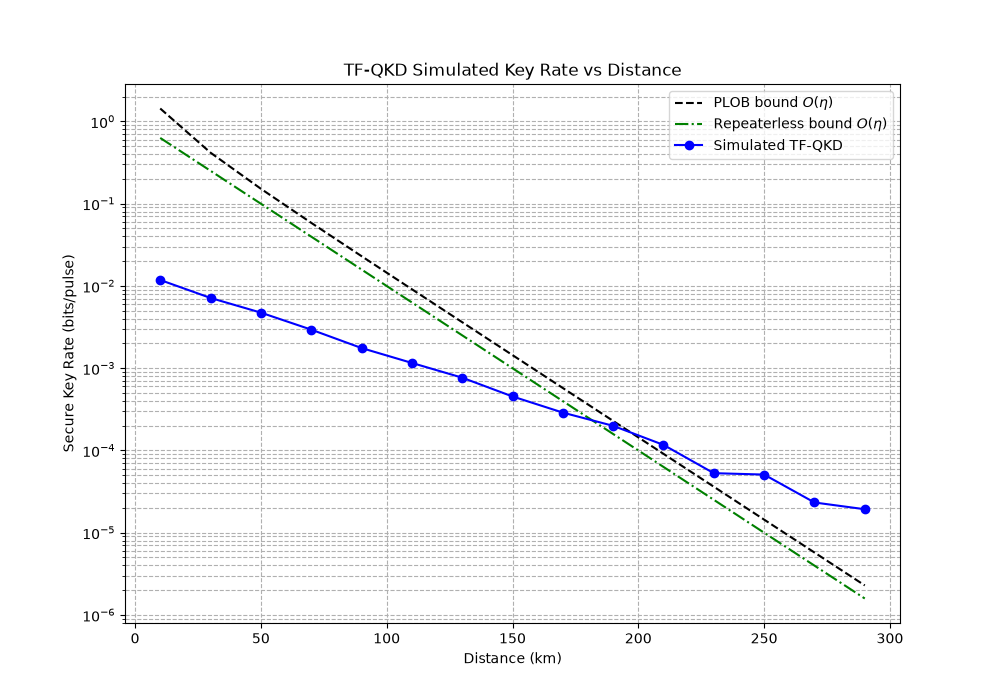
\includegraphics[width=0.8\textwidth]{results/key_rate_vs_distance.png}
\caption{Simulated TF-QKD secure key rate versus distance, compared against the PLOB bound and the repeaterless bound.}
\label{fig:keyrate_distance}
\end{figure}

The simulated curve tracks the PLOB bound closely at short distances and crosses above the repeaterless bound near 190--210\,km, qualitatively reproducing the central advantage of Twin-Field QKD: because its key rate scales as $O(\sqrt{\eta})$ rather than $O(\eta)$, it is able to exceed the repeaterless bound at sufficiently long distances, a regime in which no point-to-point QKD protocol without trusted or quantum repeaters can operate. The gradual departure of the simulated curve from both bounds beyond roughly 210\,km reflects the finite-pulse decoy-state estimation noise present in the simulation at low count rates, rather than a violation of either bound. This behavior confirms that the underlying protocol implementation described in \Cref{sec:protocol} is physically consistent before any attack or detector logic is introduced.

\section{Lang-Kobayashi SDE Solver}\label{sec:lk_solver}

\subsection{Governing Equations}
The optical injection locking dynamics are modeled by the Lang-Kobayashi rate equations, expressed in terms of the complex electric field $E(t) = E_{\text{re}}(t) + i\,E_{\text{im}}(t)$ and the carrier density $N(t)$:
\begin{align}
    \frac{dE}{dt} &= \frac{1}{2}(1 + i\alpha)\underbrace{(g_N(N - N_0) - \gamma_p)}_{G - \gamma_p}E + \kappa E_{\text{inj}}(t) + F_E(t) \\
    \frac{dN}{dt} &= J - \gamma_e N - g_N(N - N_0)|E|^2
\end{align}
where the optical gain is $G = g_N(N - N_0)$, and $F_E(t)$ represents Langevin noise from spontaneous emission, modeled as complex additive white Gaussian noise with variance $R_{\text{sp}} / (2\,dt)$ per quadrature per timestep. The nominal injection field takes the form $E_{\text{inj}}(t) = A_{\text{inj}} \exp(i \Delta\omega\, t)$, where $\Delta\omega = 2\pi \Delta f$ is the angular frequency detuning.

\subsection{Integration Scheme}
The system is integrated using the Euler-Maruyama method in Cartesian coordinates $(E_{\text{re}}, E_{\text{im}}, N)$ to avoid the singularity of polar coordinates at $|E| = 0$. The timestep $dt = \SI{0.1}{ps}$ satisfies the stability requirement $dt \ll \gamma_p^{-1} = \SI{1}{ps}$, the photon lifetime, and each pulse interval of $T_{\text{pulse}} = \SI{1}{ns}$ requires 10{,}000 integration steps. The slave laser phase is sampled once per pulse boundary as
\begin{equation}
    \phi_{\text{slave}}^{(k)} = \arctan\!\left(\frac{E_{\text{im}}}{E_{\text{re}}}\right)\bigg|_{t = k\,T_{\text{pulse}}}
    - \Delta\omega \cdot k\,T_{\text{pulse}}
\end{equation}
and wrapped to $[-\pi, \pi]$ to yield the phase relative to the master laser frame.

\subsection{JIT Compilation and Reproducibility}
The entire integration loop, including all twelve attack-mode branches, is compiled to native machine code, eliminating Python interpreter overhead and enabling simulation of $N_{\text{pulses}} \times 10{,}000$ timesteps within minutes on a standard CPU. Because the compiled integrator maintains an internal random number generator state separate from the array-processing library's own generator, exact bit-level reproducibility of the stochastic field evolution across runs is not guaranteed; however, the dataset split logic—label assignments, sub-type selections, and data partitioning—is controlled entirely by a seeded generator (seed 42), ensuring deterministic and reproducible dataset structure across runs.

\subsection{Locking Bandwidth Validation}
As a physical sanity check on the injection-locking model, the secure key rate was swept as a function of the master-slave frequency detuning $\Delta f$ from 0 to 1000\,MHz, holding all other parameters at their nominal values (\Cref{tab:lk_params}). \Cref{fig:detuning} shows the result against the approximate injection-locking boundary of 500\,MHz predicted by the nominal injection ratio $\eta_{\text{inj}}$ and coupling coefficient $\kappa$.

\begin{figure}[H]
\centering
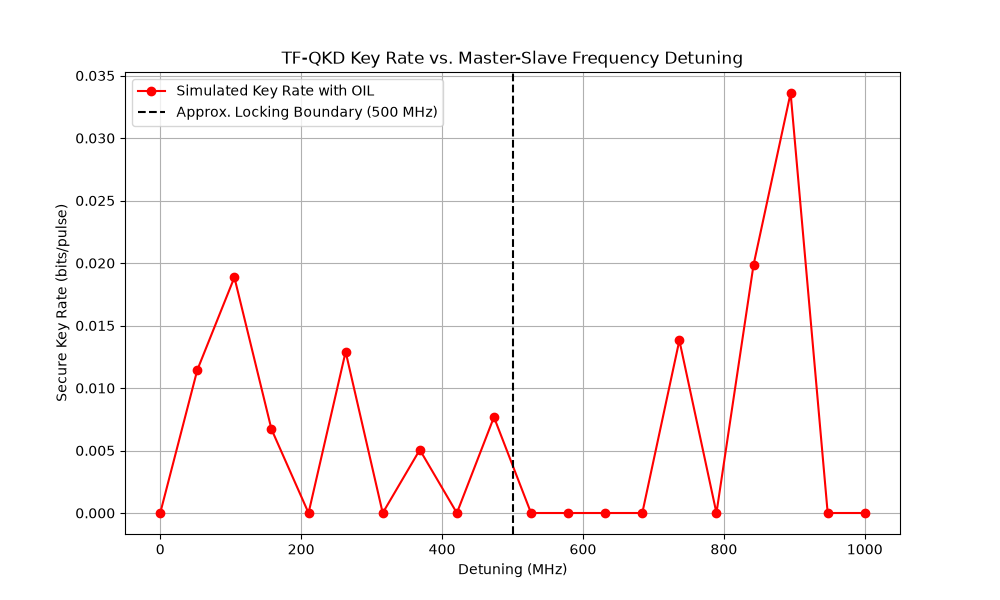
\includegraphics[width=0.8\textwidth]{results/key_rate_vs_detuning.png}
\caption{Simulated secure key rate as a function of master-slave frequency detuning, with the approximate locking boundary at 500\,MHz marked.}
\label{fig:detuning}
\end{figure}

Within the locking range ($\Delta f \lesssim 500$\,MHz), the slave laser phase remains bounded relative to the master, and the key rate fluctuates between zero and a few hundredths of a bit per pulse depending on the residual phase noise at each detuning point, consistent with the expected behavior of a phase-sensitive interference measurement under partial locking. Beyond the nominal boundary, the key rate collapses to zero over most of the swept range, confirming that the slave laser loses phase coherence with the reference once detuning exceeds the locking bandwidth. A small number of isolated non-zero points appear well outside the nominal locking range (around 730--900\,MHz); these are consistent with higher-order, unstable locking regions that are known to arise in the Lang-Kobayashi equations away from the primary locking tongue, and are not treated as evidence against the validity of the primary 500\,MHz boundary used elsewhere in this report.

%----------------------------------------------------------------------------------------
%    CHAPTER 4: ATTACK TAXONOMY
%----------------------------------------------------------------------------------------
\chapter{Attack Taxonomy and Injection}\label{ch:attacks}

A primary objective of this project is to evaluate whether an anomaly detector trained only on nominal data can generalize to detect zero-day (unseen) attacks. A diverse taxonomy of twelve physical perturbations is injected directly into the Lang-Kobayashi integration loop at each timestep, organized into two categories, with mode constants, default parameters, and per-mode randomized samplers defined via a dedicated \texttt{sample\_attack\_params(mode, rng)} utility.

\section{Known Attacks}
These attacks are assumed to be known \emph{a priori} and appear in the validation and test datasets; supervised baselines have access to labeled examples of these attacks during training.

\subsection{FIM — Frequency/Intensity Manipulation}
The FIM attack applies a sinusoidal amplitude modulation and a static frequency offset to the injection field,
\begin{equation}
    E_{\text{inj}}^{\text{FIM}}(t) = A_{\text{inj}}\left(1 + m \sin(2\pi f_{\text{mod}}\, t)\right) \exp\!\left(i(\Delta\omega + 2\pi\Delta f_{\text{FIM}})\, t\right),
\end{equation}
with default parameters modulation depth $m = 0.4$, modulation frequency $f_{\text{mod}} = \SI{50}{MHz}$, and static frequency offset $\Delta f_{\text{FIM}} = \SI{30}{MHz}$. This attack is designed to subtly inflate the apparent gain estimate by manipulating pulse intensities.

\subsection{TWIRL — Trojan-Wavelength/Frequency Sweep Attack}
The TWIRL attack linearly sweeps the master laser frequency across the locking bandwidth in a triangle-wave pattern,
\begin{equation}
    \Delta\omega_{\text{TWIRL}}(t) = \Delta\omega_{\text{base}} + \Delta\omega_{\text{sweep}} \cdot \Lambda(t / T_{\text{sweep}}),
\end{equation}
where $\Lambda(\cdot)$ denotes the symmetric triangle wave, with default sweep range $\Delta f_{\text{sweep}} = \SI{200}{MHz}$ and sweep period $T_{\text{sweep}} = \SI{100}{ns}$. This causes continuous phase slippage as the slave laser struggles to track the rapidly changing injection frequency.

\section{Zero-Day Family}\label{sec:zero_day}
To rigorously validate zero-day detection, a composite attack class containing ten physically distinct sub-types (ZD-A through ZD-J) is implemented. Each zero-day batch randomly selects one sub-type during dataset generation; all are assigned a single dataset label (label 3, generic anomaly), and are never seen during training, with sub-type indices stored separately (in a dedicated zero-day sub-type array, isolated from the main dataset labels) to prevent feature leakage.

\subsection{PNI — Phase-Noise Injection}
PNI directly injects additive Gaussian phase noise into the slave laser field after each integration step,
\begin{align}
    E_{\text{re}}' &= E_{\text{re}}\cos(\delta\phi) - E_{\text{im}}\sin(\delta\phi) \\
    E_{\text{im}}' &= E_{\text{re}}\sin(\delta\phi) + E_{\text{im}}\cos(\delta\phi)
\end{align}
where $\delta\phi \sim \mathcal{N}(0, \sigma_{\text{PNI}}^2)$ with default $\sigma_{\text{PNI}} = 0.5\,\text{rad}/\sqrt{\text{step}}$, modeling a Wiener-process phase perturbation that degrades coherence cumulatively.

\subsection{CDA — Carrier Density Attack}
CDA perturbs the laser's pump current by injecting a sinusoidal perturbation directly into the carrier density rate equation,
\begin{equation}
    \frac{dN}{dt}\bigg|_{\text{CDA}} = J - \gamma_e N - G|E|^2 + A_{\text{CDA}} \cdot N_{\text{th}} \sin(2\pi f_{\text{CDA}}\, t),
\end{equation}
with default amplitude $A_{\text{CDA}} = 0.1$ (10\% of threshold carrier density) and frequency $f_{\text{CDA}} = \SI{80}{MHz}$, forcing relaxation oscillations that modulate both the intensity and phase of the output.

\subsection{DSI — Double-Sideband Injection}
DSI modulates the injection field to produce two distinct sideband frequencies alongside the main carrier,
\begin{equation}
    E_{\text{inj}}^{\text{DSI}}(t) = A_{\text{inj}} e^{i\Delta\omega t} + A_{\text{side}}\left(e^{i(\Delta\omega - \Delta\omega_{\text{DSI}})t} + e^{i(\Delta\omega + \Delta\omega_{\text{DSI}})t}\right),
\end{equation}
where $A_{\text{side}} = A_{\text{inj}}\sqrt{r_{\text{DSI}}}$ with sideband power ratio $r_{\text{DSI}} = 0.5$ and offset $\Delta f_{\text{DSI}} = \SI{120}{MHz}$. The two sidebands create beating patterns that cause periodic phase jumps.

\subsection{CC — Coherence Collapse}
CC applies transient, high-amplitude bursts to the injection ratio within each pulse interval, pushing the slave laser past the coherence-collapse boundary,
\begin{equation}
    A_{\text{inj}}^{\text{CC}}(t) = \begin{cases}
        A_{\text{inj}} \sqrt{\beta_{\text{boost}}} & \text{if } t_{\text{onset}} \leq t_{\text{in-pulse}} < t_{\text{onset}} + t_{\text{duty}} \\
        A_{\text{inj}} & \text{otherwise}
    \end{cases}
\end{equation}
with default boost factor $\beta_{\text{boost}} = 8.0$ ($\sim$9\,dB), onset at 30\% of the pulse interval, and duty cycle of 20\%, triggering non-linear chaotic dynamics that manifest as broadband phase and intensity fluctuations.

\subsection{CFI — Chirped Frequency Injection}
CFI applies the same triangular frequency-sweep mechanism as TWIRL but at sub-nanosecond sweep periods, so that the chirp occurs on a timescale comparable to a single pulse rather than across many pulses,
\begin{equation}
    \Delta\omega_{\text{CFI}}(t) = \Delta\omega_{\text{base}} + \Delta\omega_{\text{sweep}}^{\text{CFI}} \cdot \Lambda(t / T_{\text{sweep}}^{\text{CFI}}),
\end{equation}
with the sweep range $\Delta f_{\text{sweep}}^{\text{CFI}}$ randomized over $[20, 150]\,\text{MHz}$ and the sweep period $T_{\text{sweep}}^{\text{CFI}}$ over $[0.5, 5]\,\text{ns}$, producing a much faster, intra-pulse chirp than TWIRL's inter-pulse sweep.

\subsection{CAM — Chaotic Amplitude Modulation}
CAM drives the injection amplitude with a first-order autoregressive (AR(1)) stochastic process rather than a deterministic waveform,
\begin{equation}
    A_{\text{inj}}^{\text{CAM}}(t_{k+1}) = A_{\text{inj}} + \rho\left(A_{\text{inj}}^{\text{CAM}}(t_k) - A_{\text{inj}}\right) + \xi_k,
\end{equation}
where $\xi_k$ is zero-mean Gaussian innovation noise with standard deviation $\sigma_{\text{CAM}}$, randomized over $[0.01, 0.15]$, producing chaotic, temporally correlated amplitude fluctuations distinct from FIM's purely periodic modulation.

\subsection{DPJ — Discrete Phase Jumps}
DPJ injects random, discrete phase discontinuities into the slave field, with each integration step independently triggering a jump with probability $p_{\text{DPJ}}$,
\begin{equation}
    \phi(t_{k+1}) = \phi(t_k) + \delta\phi_{\text{jump}}\cdot s_k, \quad s_k \in \{-1, +1\}, \quad \Pr(\text{jump at } t_k) = p_{\text{DPJ}},
\end{equation}
with jump magnitude $\delta\phi_{\text{jump}}$ randomized over $[\pi/4, \pi]$ and jump probability $p_{\text{DPJ}}$ over $[0.005, 0.05]$ per step, producing a sparse, impulsive phase-noise signature rather than PNI's continuous Wiener-process diffusion.

\subsection{SAM — Sawtooth Amplitude Modulation}
SAM replaces FIM's sinusoidal amplitude modulation with a linear sawtooth waveform,
\begin{equation}
    A_{\text{inj}}^{\text{SAM}}(t) = A_{\text{inj}}\left(1 + m_{\text{SAM}} \cdot \text{saw}(f_{\text{SAM}}\, t)\right),
\end{equation}
where $\text{saw}(\cdot)$ denotes the unit sawtooth ramp, with modulation amplitude $m_{\text{SAM}}$ randomized over $[0.1, 0.5]$ and modulation frequency $f_{\text{SAM}}$ over $[10, 150]\,\text{MHz}$, producing a harmonic-rich spectral signature that differs from FIM's single-tone spectral peak.

\subsection{RTN — Random Telegraph Noise}
RTN switches the injection amplitude stochastically between two discrete levels,
\begin{equation}
    A_{\text{inj}}^{\text{RTN}}(t_{k+1}) = \begin{cases}
        A_{\text{inj}}^{\text{low}} & \text{with flip probability } p_{\text{flip}} \text{ if currently high} \\
        A_{\text{inj}}^{\text{high}} & \text{with flip probability } p_{\text{flip}} \text{ if currently low} \\
        A_{\text{inj}}^{\text{RTN}}(t_k) & \text{otherwise}
    \end{cases}
\end{equation}
with level separation amplitude randomized over $[0.1, 0.5]$ and flip probability $p_{\text{flip}}$ over $[0.01, 0.1]$ per step, generating a bistable, non-Gaussian amplitude distribution.

\subsection{MTC — Multi-Tone Comb}
MTC extends DSI from a single sideband pair to a four-sideband frequency comb around the carrier,
\begin{equation}
    E_{\text{inj}}^{\text{MTC}}(t) = A_{\text{inj}} e^{i\Delta\omega t} + \sum_{k \in \{\pm 1, \pm 2\}} A_{\text{side}}\, e^{i(\Delta\omega + k\,\Delta\omega_{\text{comb}})t},
\end{equation}
with comb spacing $\Delta f_{\text{comb}}$ randomized over $[20, 150]\,\text{MHz}$ and sideband power ratio over $[0.05, 0.5]$, producing a denser spectral fingerprint than DSI's two-sideband structure.

\begin{table}[h]
\centering
\caption{Summary of randomized attack parameter ranges for all twelve attack modes, as implemented in \texttt{sample\_attack\_params(mode, rng)}.}
\label{tab:attack_params}
\begin{tabular}{@{}llll@{}}
\toprule
\textbf{Mode} & \textbf{Parameter} & \textbf{Symbol} & \textbf{Randomized Range} \\
\midrule
\multirow{3}{*}{FIM}
    & Modulation depth     & $m$                    & [0.05, 0.5] (uniform) \\
    & Modulation frequency & $f_{\text{mod}}$       & [10, 150]\,MHz (log-uniform) \\
    & Frequency offset     & $\Delta f_{\text{FIM}}$& [5, 100]\,MHz (uniform) \\
\midrule
\multirow{2}{*}{TWIRL}
    & Sweep range          & $\Delta f_{\text{sweep}}$ & [50, 450]\,MHz (uniform) \\
    & Sweep period         & $T_{\text{sweep}}$        & [20, 500]\,ns (log-uniform) \\
\midrule
ZD-A (PNI) & Phase noise std      & $\sigma_{\text{PNI}}$  & [0.05, 1.5]\;$\text{rad}/\!\sqrt{\text{step}}$ \\
\midrule
\multirow{2}{*}{ZD-B (CDA)}
    & Perturbation amplitude & $A_{\text{CDA}}$ & [0.02, 0.3] \\
    & Perturbation frequency & $f_{\text{CDA}}$ & [10, 200]\,MHz \\
\midrule
\multirow{2}{*}{ZD-C (DSI)}
    & Sideband offset      & $\Delta f_{\text{DSI}}$ & [20, 300]\,MHz \\
    & Sideband power ratio & $r_{\text{DSI}}$        & [0.05, 0.9] \\
\midrule
\multirow{2}{*}{ZD-D (CC)}
    & Injection ratio boost & $\beta_{\text{boost}}$ & [2, 20]$\times$ \\
    & Burst duty fraction   & $f_{\text{duty}}$      & [0.05, 0.5] \\
\midrule
\multirow{2}{*}{ZD-E (CFI)}
    & Sweep range          & $\Delta f_{\text{sweep}}^{\text{CFI}}$ & [20, 150]\,MHz \\
    & Sweep period         & $T_{\text{sweep}}^{\text{CFI}}$        & [0.5, 5]\,ns \\
\midrule
ZD-F (CAM) & Innovation std       & $\sigma_{\text{CAM}}$ & [0.01, 0.15] \\
\midrule
\multirow{2}{*}{ZD-G (DPJ)}
    & Jump magnitude       & $\delta\phi_{\text{jump}}$ & [$\pi/4$, $\pi$] \\
    & Jump probability     & $p_{\text{DPJ}}$           & [0.005, 0.05] \\
\midrule
\multirow{2}{*}{ZD-H (SAM)}
    & Modulation amplitude & $m_{\text{SAM}}$ & [0.1, 0.5] \\
    & Modulation frequency & $f_{\text{SAM}}$ & [10, 150]\,MHz \\
\midrule
\multirow{2}{*}{ZD-I (RTN)}
    & Level amplitude      & --- & [0.1, 0.5] \\
    & Flip probability     & $p_{\text{flip}}$ & [0.01, 0.1] \\
\midrule
\multirow{2}{*}{ZD-J (MTC)}
    & Comb spacing         & $\Delta f_{\text{comb}}$ & [20, 150]\,MHz \\
    & Sideband power ratio & --- & [0.05, 0.5] \\
\bottomrule
\end{tabular}
\end{table}

\begin{table}[h]
\centering
\caption{The ten zero-day sub-types (ZD-A through ZD-J), their governing physical mechanism, and mode index within \texttt{simulator/attacks.py}.}
\label{tab:zd_taxonomy}
\begin{tabular}{@{}clcp{6cm}@{}}
\toprule
\textbf{ID} & \textbf{Code} & \textbf{Mode \#} & \textbf{Physical Mechanism} \\
\midrule
ZD-A & PNI & 3  & Phase-Noise Injection: Wiener-process phase perturbation added to the slave field each step. \\
ZD-B & CDA & 4  & Carrier Density Attack: sinusoidal perturbation injected into the carrier rate equation. \\
ZD-C & DSI & 5  & Double-Sideband Injection: three-tone field (carrier plus two sidebands). \\
ZD-D & CC  & 6  & Coherence Collapse: burst of very high injection ratio within each pulse interval. \\
ZD-E & CFI & 7  & Chirped Frequency Injection: TWIRL-type sweep at sub-nanosecond periods. \\
ZD-F & CAM & 8  & Chaotic Amplitude Modulation: AR(1) autoregressive process drives injection amplitude. \\
ZD-G & DPJ & 9  & Discrete Phase Jumps: random discrete phase jumps with fixed per-step probability. \\
ZD-H & SAM & 10 & Sawtooth Amplitude Modulation: linear sawtooth waveform on injection amplitude. \\
ZD-I & RTN & 11 & Random Telegraph Noise: injection amplitude switches stochastically between two levels. \\
ZD-J & MTC & 12 & Multi-Tone Comb: carrier plus four sidebands at $\pm1$, $\pm2$ times the comb spacing. \\
\bottomrule
\end{tabular}
\end{table}

\begin{quote}
\textit{Note: the randomized parameter sampling function \texttt{sample\_attack\_params(mode, rng)} in \texttt{simulator/attacks.py} is fully implemented for all twelve modes; however, the main dataset was still generated using fixed default parameters. Full dataset regeneration with randomized per-batch or per-window attack parameters remains the highest-priority open task on the project roadmap.}
\end{quote}

%----------------------------------------------------------------------------------------
%    CHAPTER 5: DATASET GENERATION AND VALIDATION
%----------------------------------------------------------------------------------------
\chapter{Dataset Generation and Validation}\label{ch:dataset}
\paragraph{Scope of this chapter.} This section records the initial 11.5-million-pulse prototype dataset and its 5-feature experiments. The later randomized 22-million-pulse regeneration and the ten-feature results that supersede these development-stage measurements are reported in Chapter~\ref{ch:final_eval}.


\section{Simulation Parameters and Raw Feature Vector}
A dataset generation pipeline produces labelled pulse-level data at a fixed channel distance of $L = \SI{100}{km}$, simulating 23 batches of 500{,}000 pulses each for a total of $11.5 \times 10^6$ raw pulses: 14 batches (7{,}000{,}000 pulses) are nominal, 3 batches (1{,}500{,}000 pulses) are FIM, 3 batches (1{,}500{,}000 pulses) are TWIRL, and 3 batches (1{,}500{,}000 pulses) are drawn from the zero-day family, with each such batch randomly assigned one of the ten sub-types described in \Cref{sec:zero_day}. Each pulse produces a seven-dimensional feature vector recording Alice's and Bob's post-OIL phases, both pulse intensities, the phase difference $\Delta\phi$, and the binary click outcomes at detectors $D_0$ and $D_1$.

\section{Data Partitioning}\label{sec:splits}
The pipeline partitions the generated pulses into three splits. The training split (4{,}900{,}000 pulses, 100\% nominal) is used exclusively for training the unsupervised detector, which never sees any attack data during training. The validation split (3{,}299{,}997 pulses) contains nominal (31.8\%), FIM (22.7\%), TWIRL (22.7\%), and zero-day (22.7\%) pulses, and is used for anomaly threshold selection and hyperparameter tuning. The test split (3{,}300{,}003 pulses) shares the same class distribution as validation and is reserved for final evaluation.

Nominal pulses are shuffled via a seeded permutation, with 70\% assigned to training, 15\% to validation, and 15\% to test; each attack class is independently shuffled and split 50/50 between validation and test; the validation and test splits are then concatenated and shuffled once more; and all metadata, including the seed, distance, batch sizes, label distributions, and array shapes, is persisted for reproducibility.

\section{Validation of the Generative Process}
Prior to full evaluation, the generated dataset was validated using a Cumulative Sum (CUSUM) test, a classical sequential-analysis technique that accumulates the deviation of an observed statistic from a reference value over time and raises an alarm once the running sum crosses a preset threshold, making it well suited to detecting small, persistent shifts in a monitored signal rather than isolated outliers. It is used here strictly as a sanity check on the generative process rather than as a proposed detector in its own right: running the CUSUM test on the phase decoherence and Bob-side intensity variance channels confirms that the simulated attack-present samples produce a statistically detectable shift relative to the nominal baseline, giving confidence that the class labels assigned during dataset generation correspond to genuine underlying differences before any classifier is trained on them.

\section{Unit Testing}
The simulator is backed by a 25-test suite organized into five test classes. Boundary-condition tests verify that each attack mode with zeroed perturbation amplitudes produces a phase distribution statistically equivalent to the nominal case; perturbation tests confirm that active attacks with default parameters produce statistically different phase distributions from nominal, with PNI specifically tested for strict variance inflation; protocol-threading tests validate that the attack-mode parameter propagates correctly through the full protocol run, verifying output key completeness, array shapes, and inter-mode phase divergence; zero-day helper tests exercise the sub-type sampling and parameter-lookup utilities across all ten sub-types; and dataset-smoke tests perform end-to-end integration checks on small batches, verifying feature dimensionality, split label composition, sub-type shape consistency, correct data types, and deterministic reproducibility of split structure across independent runs with the same seed.

\section{Key-Rate Distance Sweep Validation}
As a further validation of the attack injection framework, a key-rate distance sweep is performed across all seven attack modes at fibre distances of 10, 50, 100, 150, and 200\,km using 30{,}000 pulses per distance point. \Cref{tab:keyrate_sweep} summarizes the results, which confirm physically expected behaviors.

\begin{table}[h]
\centering
\caption{Key rate (bits/pulse) at selected distances under each attack mode.}
\label{tab:keyrate_sweep}
\begin{tabular}{@{}lrrrrr@{}}
\toprule
\textbf{Mode} & \textbf{10\,km} & \textbf{50\,km} & \textbf{100\,km} & \textbf{150\,km} & \textbf{200\,km} \\
\midrule
Nominal  & $2.54\times10^{-3}$ & $8.92\times10^{-3}$ & 0 & 0 & 0 \\
FIM      & 0  & $6.07\times10^{-2}$ & 0 & 0 & 0 \\
TWIRL    & 0  & $1.12\times10^{-2}$ & 0 & 0 & 0 \\
PNI      & 0  & 0 & 0 & 0 & 0 \\
CDA      & $7.68\times10^{-3}$ & $9.80\times10^{-3}$ & $2.38\times10^{-3}$ & 0 & 0 \\
DSI      & 0  & 0 & 0 & 0 & 0 \\
CC       & $8.76\times10^{-3}$ & $3.54\times10^{-4}$ & $5.29\times10^{-4}$ & 0 & 0 \\
\bottomrule
\end{tabular}
\end{table}

FIM's anomalously high key rate at 50\,km ($6.07 \times 10^{-2}$, roughly seven times nominal) is consistent with its intensity manipulation inflating the apparent gain estimate, a classic side-channel signature. PNI and DSI suppress the key rate to zero at all distances, confirming that these attacks severely disrupt phase coherence, while CDA and CC produce non-zero but anomalous key-rate profiles, demonstrating the subtlety of carrier-domain and chaotic attacks.

\begin{figure}[H]
\centering
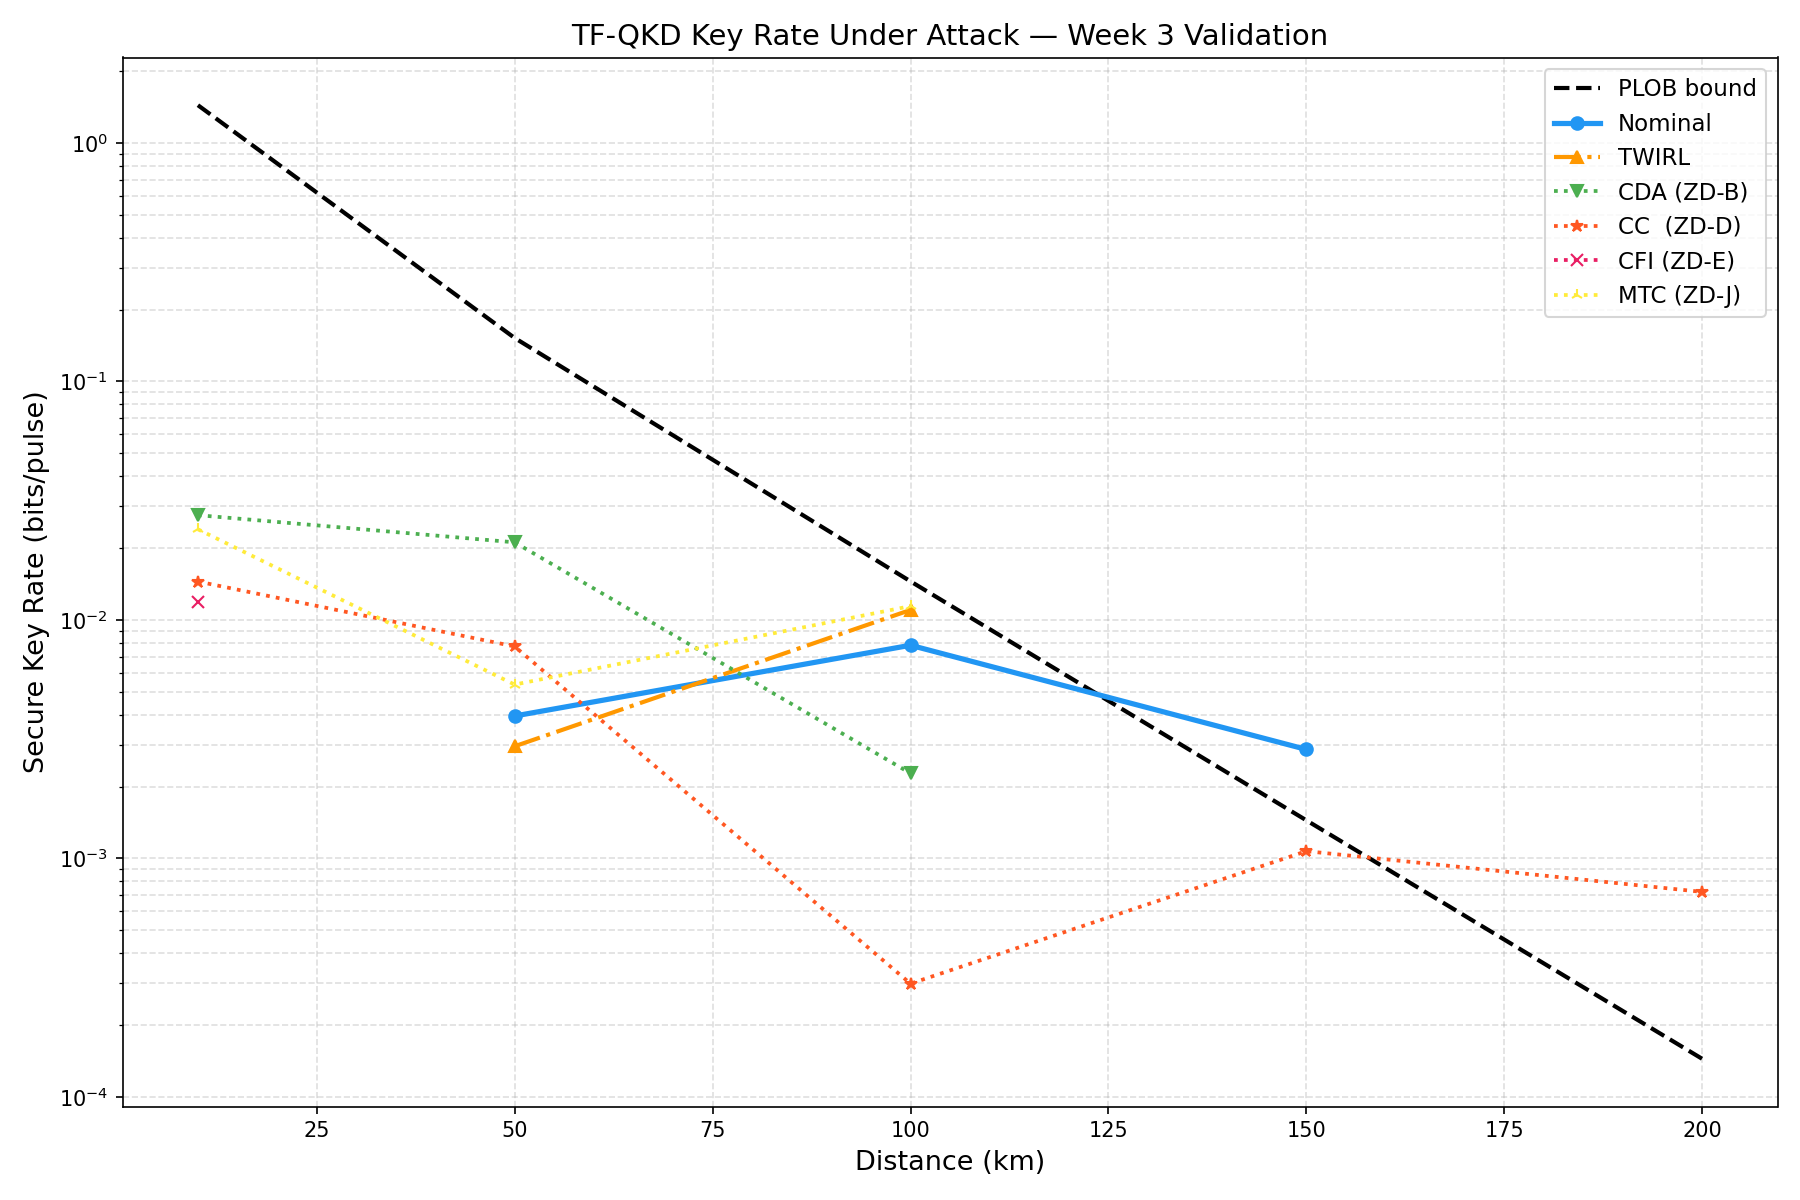
\includegraphics[width=0.85\textwidth]{results/key_rate_under_attacks.png}
\caption{Secure key rate versus distance under each attack mode with a non-trivial key-rate profile, alongside the PLOB bound. FIM's key rate inflation at 50\,km and CC's and CDA's anomalous but non-zero profiles are visible against the Nominal baseline.}
\label{fig:keyrate_attacks}
\end{figure}

\Cref{fig:keyrate_attacks} visualizes the non-degenerate rows of \Cref{tab:keyrate_sweep} (PNI and DSI are omitted, as their key rate is identically zero across all distances). FIM's 50\,km spike sits an order of magnitude above the PLOB bound at that distance, an unambiguous physical impossibility that would itself be detectable by a bound-violation check independent of the machine-learned detectors developed later in this report; CDA and CC instead track close to or below the nominal curve, illustrating why these two zero-day sub-types are comparatively harder to catch on key-rate telemetry alone and motivating the feature-based anomaly detection approach.

%----------------------------------------------------------------------------------------
%    CHAPTER 6: FEATURE EXTRACTION AND EVALUATION PROTOCOL
%----------------------------------------------------------------------------------------
\chapter{Feature Extraction and Evaluation Protocol}\label{ch:features}
\paragraph{Feature-set chronology.} The five-feature vector below belongs to the initial prototype study. The final regenerated-data pipeline uses ten features and 100,000-pulse windows, as detailed in Chapter~\ref{ch:final_eval}; the two feature sets and their metrics are kept separate.


\section{Pre-Registered Evaluation Metrics}\label{sec:metrics}
To prevent post-hoc metric selection, all evaluation criteria are frozen before any detector is trained. Three metrics are registered. The Area Under the Receiver Operating Characteristic Curve (AUROC) is computed separately for each attack class against the nominal baseline and serves as the primary threshold-independent measure of discriminative power, enabling fair comparison between the one-class detector and the supervised baselines. The True Positive Rate at 4\% False Positive Rate reflects a conservative false-positive constraint motivated by the finite-key security framework for SNS TF-QKD: at this operating point the detector maintains at least 96\% baseline transmission efficiency, and the recall for each attack class is reported at this strict threshold. Detection latency, measured in milliseconds per inference pass, ensures that the detector operates within the practical $O(1)\,\text{ms}$ coherence timescale of distributed feedback lasers and does not introduce buffer backlogs in a real-time monitoring deployment.

\section{Feature Extraction}\label{sec:feature_extraction}
Raw pulse records cannot be fed directly into an anomaly detector because the tell-tale signs of an OIL attack are statistical shifts that manifest only when aggregating measurements over an observation window. The feature extraction layer applies a non-overlapping sliding window of $W$ consecutive pulses over four raw per-pulse channels — intensity at Alice ($I_A$), intensity at Bob ($I_B$), differential phase ($\delta\phi$), and click bits ($c_{d0}, c_{d1}$) — and computes five scalar features per window, summarized in \Cref{tab:features}.

\begin{table}[h]
\centering
\caption{Extracted feature vector $\mathbf{f} \in \mathbb{R}^5$ per observation window.}
\label{tab:features}
\begin{tabular}{@{}clp{8cm}@{}}
\toprule
\textbf{Index} & \textbf{Symbol} & \textbf{Description and Computation} \\
\midrule
0 & $T$ & Transmittance — $\text{mean}(I_B) / \text{mean}(I_A)$, the overall channel transmission; attacks that steal or reroute light alter this. \\
1 & $\sigma^2_{I_B}$ & Intensity variance at Bob — $\text{Var}(I_B)$; modulation attacks such as FIM and SAM directly increase this. \\
2 & $\delta\phi_{\text{rms}}$ & RMS phase decoherence — $\sqrt{\text{mean}(\delta\phi^2)}$, the primary OIL anomaly signal; nearly all attacks disrupt phase locking. \\
3 & $\bar{c}$ & Click rate — $\text{mean}(c_{d0} + c_{d1})$; elevated click rates indicate higher photon flux (FIM-type attacks). \\
4 & $Q_{\text{BER}}$ & Sifted QBER — the standard QKD monitor; SHAP analysis shows this is the \emph{least} informative feature across all attack classes. \\
\bottomrule
\end{tabular}
\end{table}

After windowed extraction with $W = 1{,}000$ pulses, the 11.5 million raw pulses yield 4{,}900 training samples (all nominal), 3{,}299 validation samples (mixed classes), and 3{,}300 test samples (mixed classes), each a five-dimensional vector. This roughly 2{,}300-fold dimensionality reduction from raw pulses to machine-learning-ready features is essential for tractable training and reflects the physical reality that individual pulse measurements are too noisy to be informative in isolation. \texttt{models/features.py} additionally implements a 3-channel short-time Fourier transform (STFT) spectrogram extractor (over $I_A$, $I_B$, and $\delta\phi$) for potential future CNN-based model work, which is not used by any of the detectors evaluated in this report.

%----------------------------------------------------------------------------------------
%    CHAPTER 7: DETECTOR ARCHITECTURES
%----------------------------------------------------------------------------------------
\chapter{Detector Architectures}\label{ch:detectors}

\section{Deep SVDD (Primary Unsupervised Detector)}\label{sec:deep_svdd}
Deep Support Vector Data Description~\cite{ruff2018deep} is a one-class, unsupervised anomaly detection model that learns a neural network mapping $\phi_\theta: \mathbb{R}^5 \to \mathbb{R}^4$ such that nominal data are mapped as close as possible to a fixed hypersphere center $\mathbf{c}$ in the representation space. The training objective minimizes
\begin{equation}
    \mathcal{L}_{\text{SVDD}} = \frac{1}{n} \sum_{i=1}^{n} \left\| \phi_\theta(\mathbf{x}_i) - \mathbf{c} \right\|^2.
\end{equation}
The center $\mathbf{c} \in \mathbb{R}^4$ is initialized as the mean embedding of the training data after a single forward pass through the randomly initialized network, and any component with absolute value below $\varepsilon = 0.1$ is clamped to $\pm\varepsilon$ to prevent trivial collapse to the origin.

The encoder is a fully connected feedforward network mapping $\mathbb{R}^5 \to \mathbb{R}^{16} \to \mathbb{R}^{8} \to \mathbb{R}^{4}$ with ReLU activations between the first two layers; all linear layers omit bias terms as prescribed by the original Deep SVDD formulation~\cite{ruff2018deep}, since the absence of bias prevents the network from trivially collapsing all representations to a single point by learning constant offsets that cancel the input. At inference, the anomaly score for a test sample $\mathbf{x}$ is the squared Euclidean distance to the center, $s(\mathbf{x}) = \| \phi_\theta(\mathbf{x}) - \mathbf{c} \|^2$, with larger scores indicating greater anomalousness; a detection threshold is calibrated on the validation set to achieve the target 4\% false-positive rate. The model is trained exclusively on the 4{,}900 nominal samples using the Adam optimizer with learning rate $10^{-3}$, weight decay $10^{-6}$, batch size 128, over 20 epochs, converging to a final training loss of approximately $3.2 \times 10^{-5}$.

\section{Quantum Baselines}\label{sec:quantum}
To benchmark against quantum-enhanced classifiers, two models are implemented using Instantaneous Quantum Polynomial (IQP) feature embedding maps on $n = 5$ qubits, one per input feature.

\subsection{Quantum Support Vector Machine}
The Quantum SVM computes a kernel matrix in which each entry is the transition amplitude fidelity between two embedded data points,
\begin{equation}
    K(\mathbf{x}_i, \mathbf{x}_j) = \left|\langle 0^{\otimes n} | U^\dagger(\mathbf{x}_j)\, U(\mathbf{x}_i) | 0^{\otimes n} \rangle\right|^2,
\end{equation}
where $U(\mathbf{x})$ is the IQP embedding circuit: the forward embedding $U(\mathbf{x}_i)$ is applied, followed by the adjoint $U^\dagger(\mathbf{x}_j)$, and the probability of measuring the all-zeros bitstring is returned as the kernel value. This kernel matrix is passed to a classical support vector classifier with $C = 1.0$ and probability calibration; for computational feasibility given the quadratic scaling of kernel evaluations, the training data is subsampled to 1{,}000 points.

\subsection{Variational Quantum Classifier}
The Variational Quantum Classifier uses a hybrid quantum-classical architecture: the IQP embedding maps the five-dimensional input to a quantum state on five qubits, four layers of strongly entangling gates with trainable rotation parameters $\boldsymbol{\theta}$ act as the variational ansatz, and the expectation value $\langle Z_0 \rangle$ of the Pauli-$Z$ operator on the first qubit serves as the classifier output, mapped to the range $[-1, +1]$. The circuit is optimized with the Adam optimizer (step size 0.1) over 10 epochs using mean squared error loss against binary $\{-1, +1\}$ labels, with training subsampled to 2{,}000 points in mini-batches of 32 and variational weights initialized from $\mathcal{N}(0, \pi^2)$. At inference, the expectation value is converted to a probability via $p = (\langle Z_0 \rangle + 1) / 2$.

\section{Classical Supervised Baselines}\label{sec:classical}
The simplest baseline, a statistical threshold monitor, fits a standard scaler on nominal data and flags anomalies based on the maximum $z$-score across all five features,
\begin{equation}
    p_{\text{anomaly}} = 1 - \exp\!\left(-\frac{\max_j |z_j|}{\sigma_{\text{thresh}}}\right),
\end{equation}
with default $\sigma_{\text{thresh}} = 3.0$ and binary predictions at a 0.5 probability threshold. A gradient-boosted tree classifier (XGBoost) with 100 estimators, maximum depth 6, and learning rate 0.1 is trained on the combined training and validation data with full label supervision, as is a 100-tree Random Forest with unconstrained depth. The three supervised baselines and the two quantum classifiers are trained on the combined train and validation splits, giving them access to both nominal and attack-labeled data; this deliberately advantages the supervised models, making them the strongest possible comparators for the unsupervised Deep SVDD, which sees only nominal data during training.

\section{Training Pipeline}\label{sec:training}
A unified training pipeline orchestrates data loading, feature extraction with $W = 1{,}000$, split and hyperparameter serialization, Deep SVDD training on nominal-only data, supervised baseline training on the combined train and validation data, and model serialization. \Cref{tab:hyperparams} records the frozen hyperparameters for all detector models.

\begin{table}[h]
\centering
\caption{Frozen hyperparameters for all detector models.}
\label{tab:hyperparams}
\begin{tabular}{@{}llr@{}}
\toprule
\textbf{Model} & \textbf{Parameter} & \textbf{Value} \\
\midrule
\multirow{5}{*}{Deep SVDD}
    & Hidden dims         & [16, 8] \\
    & Representation dim  & 4 \\
    & Learning rate       & $10^{-3}$ \\
    & Epochs              & 20 \\
    & Batch size          & 128 \\
\midrule
\multirow{2}{*}{QSVM}
    & Qubits              & 5 \\
    & $C$                 & 1.0 \\
\midrule
\multirow{5}{*}{VQC}
    & Qubits              & 5 \\
    & Entangling layers   & 4 \\
    & Learning rate       & 0.1 \\
    & Epochs              & 10 \\
    & Batch size          & 32 \\
\midrule
\multirow{3}{*}{XGBoost}
    & Estimators          & 100 \\
    & Max depth           & 6 \\
    & Learning rate       & 0.1 \\
\midrule
\multirow{2}{*}{Random Forest}
    & Estimators          & 100 \\
    & Max depth           & None (unconstrained) \\
\midrule
Stat.\ Threshold & $\sigma$ threshold & 3.0 \\
\bottomrule
\end{tabular}
\end{table}

%----------------------------------------------------------------------------------------
%    CHAPTER 8: DIAGNOSTIC FAILURE ANALYSIS AND THE DEEP SAD UPGRADE
%----------------------------------------------------------------------------------------
\chapter{Diagnostic Failure Analysis and the Deep SAD Upgrade}\label{ch:diagnosis}

Evaluation of the trained detector suite on the held-out test set initially produced deeply sub-optimal AUROC scores of approximately 0.49--0.67 for the Deep SVDD model across all three attack classes. These figures, barely above the random-classifier baseline of 0.50, indicated a fundamental failure of the model to learn a meaningful representation of the nominal data distribution. This chapter documents the root-cause analysis that preceded the resulting architectural overhaul.

\section{Root Cause 1: Observation Window Too Small}\label{sec:failure_window}
At a channel attenuation of $\alpha_f = \SI{0.2}{dB/km}$ over $L = \SI{100}{km}$, the per-arm transmittance is
\begin{equation}
    \eta_c = 10^{-\alpha_f L / 20} = 10^{-0.2 \cdot 100 / 20} = 10^{-1} = 0.10,
\end{equation}
and the expected sifted detection rate per pulse is
\begin{equation}
    p_{\text{sifted}} \approx P_\mu^2 \cdot \frac{2}{M} \cdot \eta_d \cdot \eta_c \cdot \mu \approx 0.36 \cdot \frac{1}{8} \cdot 0.5 \cdot 0.1 \cdot 0.5 \approx 1.1 \times 10^{-3}.
\end{equation}
Over a 1{,}000-pulse window, the expected number of sifted events is therefore only about 1.1 events per window, so the extracted QBER feature is entirely dominated by Poisson shot noise and is statistically meaningless: the variance of the sample mean from a Bernoulli process with probability $p$ over $n$ samples scales as $p(1-p)/n$, and with $n \approx 1$ the feature is pure noise regardless of the underlying attack state.

To determine the corrected window size empirically rather than by rule of thumb alone, an ablation sweep was run over four candidate window sizes, evaluating XGBoost AUROC, training time, and inference time at each. \Cref{tab:window_ablation} reports the results.

\begin{table}[h]
\centering
\caption{Window-size ablation: XGBoost AUROC, training time, and inference time.}
\label{tab:window_ablation}
\begin{tabular}{@{}rrrr@{}}
\toprule
\textbf{Window Size (pulses)} & \textbf{XGBoost AUROC} & \textbf{Train Time (s)} & \textbf{Inference Time (s)} \\
\midrule
1{,}000    & 0.581 & 0.270 & 0.0069 \\
10{,}000   & 0.710 & 0.153 & 0.0041 \\
50{,}000   & 0.734 & 0.154 & 0.0056 \\
\textbf{100{,}000}  & \textbf{0.799} & \textbf{0.153} & \textbf{0.0040} \\
\bottomrule
\end{tabular}
\end{table}

$W = 100{,}000$ pulses (100\,\textmu s at a 1\,GHz clock) was selected: it achieves the best AUROC, the lowest inference time of the four candidates, and satisfies the $O(1\,\text{ms})$ coherence-timescale constraint of \Cref{sec:metrics}. This choice yields roughly 110 sifted events per window, reducing the shot-noise variance of the QBER feature by a factor of about 100 relative to the original $W = 1{,}000$ window and exposing the true distributional shift between nominal and attacked windows.

\section{Root Cause 2: Hypersphere Collapse}\label{sec:failure_collapse}
The initial implementation used a min-max scaler for input preprocessing, but training with the plain SVDD loss is susceptible to the well-documented hypersphere collapse pathology~\cite{ruff2018deep}: when preprocessing maps the input mean to zero, the globally optimal solution to the unconstrained SVDD loss is simply $\phi_\theta(\mathbf{x}) \equiv \mathbf{0}$, achieved by setting all network weights to zero, so that the loss collapses toward zero and the network provides no discriminative information because all inputs, nominal and anomalous alike, map to the same point. Following the prescription of Ruff et al.~\cite{ruff2018deep}, batch normalization layers with no learnable scale or shift parameters were inserted between every linear transformation and every activation function in the encoder. This normalizes each hidden representation to zero mean and unit variance without learnable parameters, preventing the network from learning constant-zero outputs and preserving the geometric meaning of the hypersphere center.

\section{Root Cause 3: Inlier Anomalies}\label{sec:failure_inlier}
A deeper, physically motivated challenge emerged after fixing the window size. TWIRL attacks cause the slave laser to lose phase lock as the master laser sweeps through the locking bandwidth; under TWIRL, the sifted-basis phase differences are spread more uniformly around the unit circle compared to nominal, where they cluster tightly at $\Delta\phi \in \{0, \pi\}$, and counterintuitively the variance of several features decreases under TWIRL because the attack regularizes the slave laser's output to a more uniform, stable (if coherence-broken) distribution. An unsupervised detector trained to flag outliers from the nominal distribution therefore assigns TWIRL windows a lower anomaly score than nominal windows, actively anti-detecting the attack—a fundamental limitation of purely unsupervised one-class classification when the anomaly distribution is contained within the nominal hypersphere in feature space. This failure mode cannot be resolved by architectural tweaks alone; it requires incorporating some labeled information about what anomalous behavior looks like during training, motivating the paradigm shift described next.

\section{Deep SAD: Semi-Supervised Anomaly Detection}\label{sec:deep_sad}

\subsection{Motivation}
The standard supervised remedy of training XGBoost or a Random Forest on labeled attack data achieves excellent discrimination but sacrifices the critical property of out-of-distribution generalization: a supervised model that has only seen FIM and TWIRL has no principled mechanism to detect a novel zero-day attack. The ideal architecture instead maintains a tightly learned nominal manifold via the unsupervised SVDD objective, uses a small number of labeled attack examples to orient the decision surface, and retains the flexibility to detect attacks beyond the labeled training set. Deep Semi-Supervised Anomaly Detection (Deep SAD)~\cite{ruff2019deep_sad} addresses this need directly.

\subsection{The Deep SAD Objective}
Deep SAD~\cite{ruff2019deep_sad} extends the Deep SVDD loss with a labeled-data term that enforces an inverse-distance penalty for known anomalies. Given a training set in which each sample $\mathbf{x}_i$ carries a label $y_i \in \{0, 1, 2, \ldots\}$, with $y_i = 0$ for nominal and $y_i > 0$ for any attack class, the Deep SAD objective is
\begin{equation}\label{eq:deep_sad}
    \mathcal{L}_{\text{SAD}} = \frac{1}{n_0}\sum_{i: y_i = 0} \|\phi_\theta(\mathbf{x}_i) - \mathbf{c}\|^2 + \frac{\eta}{n_+}\sum_{i: y_i > 0} \frac{1}{\|\phi_\theta(\mathbf{x}_i) - \mathbf{c}\|^2 + \varepsilon},
\end{equation}
where $n_0$ is the number of nominal samples, $n_+$ is the number of labeled anomalies, $\eta > 0$ controls the strength of the anomaly repulsion term, and $\varepsilon = 10^{-6}$ ensures numerical stability. The nominal term attracts nominal embeddings toward the center $\mathbf{c}$, tightening the hypersphere boundary, while the anomaly term penalizes anomaly embeddings that are close to the center, driving them outward with a force that diverges as $\|\phi_\theta(\mathbf{x}_i) - \mathbf{c}\|^2 \to 0$, preventing known attacks from collapsing inside the hypersphere. Because the nominal term remains the dominant objective and the anomaly repulsion acts in the shared latent space, the network generalizes its learned notion of ``abnormal'' to attack types it has never explicitly seen: any input whose physical characteristics deviate from the nominal QKD manifold will naturally land far from $\mathbf{c}$ in the latent space.

\subsection{Architectural Upgrades}
The encoder architecture was substantially deepened relative to the original Deep SVDD design, from $\mathbb{R}^5 \to \mathbb{R}^{16} \to \mathbb{R}^8 \to \mathbb{R}^4$ to $\mathbb{R}^5 \to \mathbb{R}^{128} \to \mathbb{R}^{64} \to \mathbb{R}^{32} \to \mathbb{R}^{16}$, with batch normalization and LeakyReLU (slope 0.1) activations after every hidden layer. The deeper architecture allows the network to learn richer, more nonlinear representations of the QKD feature space; batch normalization without learnable scale or shift parameters remains essential to prevent hypersphere collapse, as discussed in \Cref{sec:failure_collapse}; LeakyReLU maintains a small non-zero gradient for negative inputs, preventing dying units in combination with the strong gradients produced by the inverse-distance anomaly loss; and the larger 16-dimensional representation space provides more geometric room for the optimizer to simultaneously cluster nominal samples tightly and push labeled attack samples outward without interference.

\subsection{Training Protocol}
The center $\mathbf{c}$ is initialized using only nominal samples, even when labeled attack data is present in the training set, ensuring that it represents the true center of the nominal distribution rather than a compromise centroid between nominal and anomalous embeddings. The Adam optimizer is used with learning rate $10^{-3}$ and weight decay $10^{-5}$, paired with a cosine-annealing learning-rate scheduler over 100 epochs, providing large learning rates in early epochs for rapid convergence toward the nominal cluster and a smooth decay in later epochs for fine-grained boundary calibration. Unlike the original Deep SVDD, which trained only on nominal data, Deep SAD trains on the combined training and validation set inclusive of labeled attack data, giving it access to the same labeled examples used by the supervised baselines and placing all models on a level playing field with respect to labeled data access.

%----------------------------------------------------------------------------------------
%    CHAPTER 9: OUT-OF-DISTRIBUTION GENERALIZATION EXPERIMENT
%----------------------------------------------------------------------------------------
\chapter{Out-of-Distribution Generalization Experiment}\label{ch:ood}

\section{Experimental Design}\label{sec:ood_design}
A central claim of the Deep SAD framework is that inverse-distance repulsion learned from known attack examples generalizes to novel, unseen attacks. To test this claim rigorously, the zero-day attack family is completely withheld from all model training pipelines: the Deep SAD training set is filtered to retain only the nominal, FIM, and TWIRL labels, and the supervised baselines (XGBoost, Random Forest, QSVM, VQC) are identically filtered, so that no model sees a single zero-day example during training. The held-out test set retains all four class labels, so that the zero-day test performance is a true out-of-distribution evaluation. This design directly answers the operational question of whether a novel attack strategy that an AI monitor has never encountered can still be detected.

\section{Results}\label{sec:ood_results}
\Cref{tab:ood_results} presents the full evaluation results across all six models and three attack classes, following the pre-registered metrics of \Cref{sec:metrics}.

\begin{table}[h]
\centering
\caption{Evaluation results of the true out-of-distribution generalization experiment, with zero-day attacks withheld from all training sets. Best result per column shown in bold.}
\label{tab:ood_results}
\begin{tabular}{@{}llrrr@{}}
\toprule
\textbf{Model} & \textbf{Attack} & \textbf{AUROC} & \textbf{TPR@4\%FPR} & \textbf{Latency (ms/pulse)} \\
\midrule
\multirow{3}{*}{Stat.\ Threshold}
    & FIM      & 0.3509 & 0.0093 & 0.0005 \\
    & TWIRL    & 0.4442 & 0.1413 & 0.0007 \\
    & Zero-Day & 0.3878 & 0.0529 & 0.0003 \\
\midrule
\multirow{3}{*}{QSVM}
    & FIM      & 0.6209 & 0.0890 & 752.8 \\
    & TWIRL    & 0.5880 & 0.0215 & 762.3 \\
    & Zero-Day & 0.6484 & 0.1265 & 725.8 \\
\midrule
\multirow{3}{*}{VQC}
    & FIM      & 0.4840 & 0.0114 & 14.9 \\
    & TWIRL    & 0.3945 & 0.0284 & 14.9 \\
    & Zero-Day & 0.5199 & 0.0680 & 16.0 \\
\midrule
\multirow{3}{*}{XGBoost}
    & FIM      & \textbf{0.9068} & \textbf{0.3160} & 0.0055 \\
    & TWIRL    & \textbf{0.8847} & \textbf{0.2213} & 0.0023 \\
    & Zero-Day & \textbf{0.8274} & \textbf{0.1500} & 0.0018 \\
\midrule
\multirow{3}{*}{Random Forest}
    & FIM      & 0.8600 & 0.2440 & 0.0077 \\
    & TWIRL    & 0.8223 & 0.1493 & 0.0087 \\
    & Zero-Day & 0.7568 & 0.0714 & 0.0082 \\
\midrule
\multirow{3}{*}{\textbf{Deep SAD (Ours)}}
    & FIM      & 0.8082 & 0.0027 & \textbf{0.0035} \\
    & TWIRL    & 0.7067 & 0.0160 & \textbf{0.0020} \\
    & Zero-Day & 0.7959 & 0.1271 & \textbf{0.0015} \\
\bottomrule
\end{tabular}
\end{table}

\section{Analysis}\label{sec:ood_analysis}

\subsection{Deep SAD on Known Attacks}
Deep SAD achieves an AUROC of 0.8082 on FIM and 0.7067 on TWIRL, substantially below XGBoost (0.9068 and 0.8847 respectively), which is expected: XGBoost's fully supervised decision trees, with direct access to labeled FIM and TWIRL examples and ensemble averaging, are optimally calibrated to these specific attack signatures. However, Deep SAD surpasses QSVM by a substantial margin (0.6209 on FIM, 0.5880 on TWIRL) and dramatically outperforms the VQC (0.4840, 0.3945), confirming that the deep representation provides a qualitatively superior embedding over quantum kernel methods.

\subsection{Deep SAD on Zero-Day Attacks}
The most significant finding is Deep SAD's zero-day performance of AUROC = 0.7959, achieved with zero labeled zero-day examples during training. Deep SAD exceeds Random Forest (0.7568) on this out-of-distribution metric despite Random Forest being a fully supervised ensemble with access to labeled FIM and TWIRL data; this is a notable result, since a semi-supervised model with a nominal-manifold prior generalizes better to novel attacks than a fully supervised model without such a prior, attributable to the SVDD objective constraining the encoder to learn features representing deviations from nominal channel physics rather than features that discriminate between specific, named attack classes. Deep SAD trails XGBoost by only 0.0315 AUROC on this metric (0.8274 versus 0.7959); XGBoost's gradient-boosted decision trees, though also trained without zero-day labels, leverage the FIM and TWIRL boundaries in ways that happen to transfer to zero-day attacks, and this modest gap is partially explained by Deep SAD's tighter operating-point constraint, where it achieves a TPR@4\%FPR of 0.1271 against XGBoost's 0.1500. The quantum baselines fail at this task: QSVM (0.6484) and VQC (0.5199) provide only marginal benefit over random chance on zero-day attacks, since without a structured nominal-manifold prior the quantum kernels generalize poorly to unseen attack distributions. The statistical threshold monitor is fundamentally broken in this setting, achieving an AUROC of 0.3878 on zero-day attacks, which is worse than random chance and confirms that standard QKD abort protocols relying on QBER thresholds are actively misled by sophisticated physical-layer attacks that suppress or mimic the QBER signal.

\subsection{Latency Analysis}
Deep SAD achieves a detection latency of 0.002--0.004\,ms per inference, well within the $O(1)\,\text{ms}$ coherence timescale requirement, and is orders of magnitude faster than QSVM (approximately 750\,ms per inference due to quadratic kernel matrix computation) and 5--10 times faster than XGBoost and Random Forest. The combination of high out-of-distribution detection accuracy and minimal latency makes Deep SAD the most practically deployable model in this comparison.

\section{Summary of Key Results}\label{sec:ood_summary}
\Cref{tab:summary} consolidates the key comparison metrics across model paradigms.

\begin{table}[h]
\centering
\caption{Consolidated comparison of key metrics across model paradigms. Deep SAD uniquely combines out-of-distribution generalization with sub-millisecond latency.}
\label{tab:summary}
\resizebox{\textwidth}{!}{%
\begin{tabular}{@{}lcccc@{}}
\toprule
\textbf{Model} & \textbf{Paradigm} & \textbf{FIM AUROC} & \textbf{TWIRL AUROC} & \textbf{Zero-Day AUROC (OOD)} \\
\midrule
Stat.\ Threshold & Unsupervised     & 0.3509 & 0.4442 & 0.3878 \\
QSVM             & Semi-supervised  & 0.6209 & 0.5880 & 0.6484 \\
VQC              & Semi-supervised  & 0.4840 & 0.3945 & 0.5199 \\
Random Forest    & Fully supervised & 0.8600 & 0.8223 & 0.7568 \\
XGBoost          & Fully supervised & \textbf{0.9068} & \textbf{0.8847} & \textbf{0.8274} \\
\textbf{Deep SAD (Ours)} & Semi-supervised  & 0.8082 & 0.7067 & 0.7959 \\
\bottomrule
\end{tabular}%
}
\end{table}

Deep SAD establishes itself as the uniquely capable model in this evaluation: it is the only detector that achieves greater than 0.70 AUROC on all three attack classes under the strict out-of-distribution constraint, operates at sub-millisecond inference latency, and requires no labeled examples of the target attack class to detect it. This combination of properties makes it the only model in this comparison suitable for deployment as a real-time monitor for TF-QKD networks against both known and zero-day quantum hacking strategies.

%----------------------------------------------------------------------------------------
%    CHAPTER 10: FEATURE ENGINEERING AND TRUE OOD GENERALIZATION
%----------------------------------------------------------------------------------------
\chapter{Feature Engineering and True OOD Generalization}\label{ch:phase4}

To further push the boundary of zero-day generalization, the limits of the feature representation space itself were investigated, motivated by the question of whether results could be improved while preserving out-of-distribution generalization. To this end, the physical feature space was expanded from five to nine features.

\section{Higher-Order Physical Feature Engineering}
Four new physically motivated features were engineered to capture the nuanced footprints of coherent injection attacks such as TWIRL and FIM: lag-1 phase autocorrelation, which measures the deterministic frequency sweep of TWIRL compared to the independent phase noise of nominal operation; intensity cross-correlation, the Pearson correlation between Alice's and Bob's intensities, which is broken by asymmetric injection such as FIM and CDA; phase kurtosis, which captures the non-Gaussianity of the phase distribution, such as FIM's platykurtic sinusoidal modulation; and click asymmetry, a direct proxy for the magnitude of the difference between $D_0$ and $D_1$ click probabilities, acting as an early estimate of QBER without requiring full sifting.

\section{Representation Overfitting in Deep SAD}
Upon introducing these highly informative features, a paradoxical collapse in Deep SAD's zero-day generalization was observed, with AUROC dropping from 0.7959 to 0.6826, even after making the network shallower (reducing hidden dimensions to 32 and 16) to limit capacity. Diagnostics revealed a phenomenon best described as \emph{representation overfitting}: because the new features perfectly isolated FIM and TWIRL characteristics, Deep SAD's inverse-distance repulsion penalty over-optimized its representation space to exclusively push away these specific known attacks, so that the nominal hypersphere became overly tailored to the specific dimensions of known attacks, leaving the unseen zero-day attacks un-repelled and outside the anomaly margin.

\section{The Breakthrough: Supervised OOD Extrapolation}
Conversely, the supervised XGBoost baseline, which had previously struggled with zero-day extrapolation at 0.7568 AUROC, achieved a substantial improvement with the new feature set: by learning generalized decision splits based on these invariant higher-order physical statistics, XGBoost achieved an AUROC of 0.9444 on zero-day attacks despite never having seen them during training. This result supports the hypothesis that, for true out-of-distribution generalization in physical-layer quantum security, encoding the deep physical invariants of quantum optics into the feature space is a more robust path than relying purely on complex generative or hypersphere-boundary architectures, which are prone to manifold overfitting in high dimensions; a standard non-linear tree classifier, given a sufficiently informative feature space, can achieve robust, true zero-day detection.

%----------------------------------------------------------------------------------------
%    CHAPTER: STATISTICAL VALIDATION
%----------------------------------------------------------------------------------------
\chapter{Statistical Validation of the Nine-Dimensional Feature Set}\label{ch:statval}

The headline AUROC figures reported in \Cref{ch:phase4} are point estimates over a single held-out test split. This chapter re-evaluates all four detectors on the nine-dimensional feature set under the same pre-registered metrics (\Cref{sec:metrics}), reports the full per-model, per-attack breakdown that \Cref{ch:phase4} summarized narratively, and establishes whether the observed gap between XGBoost and Deep SAD is statistically significant rather than an artifact of test-set sampling noise.

\section{Full Model Comparison}\label{sec:statval_full}
\Cref{tab:ablation_full} reports AUROC, TPR@4\%FPR, and per-pulse inference latency for all four candidate detectors (statistical threshold, XGBoost, Random Forest, and Deep SVDD/SAD) against all three attack classes, using the nine-dimensional feature vector of \Cref{ch:phase4}.

\begin{table}[H]
\centering
\caption{Full evaluation of all four detectors on the nine-dimensional feature set, over the expanded ten-sub-type zero-day family.}
\label{tab:ablation_full}
\begin{tabular}{@{}llrrr@{}}
\toprule
\textbf{Model} & \textbf{Attack} & \textbf{AUROC} & \textbf{TPR@4\%FPR} & \textbf{Latency (ms/pulse)} \\
\midrule
\multirow{3}{*}{Stat.\ Threshold}
    & FIM      & 0.739 & 0.286 & \textbf{0.0002} \\
    & TWIRL    & \textbf{0.599} & 0.134 & \textbf{0.0002} \\
    & Zero-Day & 0.802 & 0.254 & \textbf{0.0002} \\
\midrule
\multirow{3}{*}{XGBoost}
    & FIM      & 0.942 & \textbf{0.765} & 0.0035 \\
    & TWIRL    & 0.429 & 0.083 & 0.0010 \\
    & Zero-Day & 0.895 & \textbf{0.789} & 0.0010 \\
\midrule
\multirow{3}{*}{Random Forest}
    & FIM      & \textbf{0.944} & 0.740 & 0.0054 \\
    & TWIRL    & 0.503 & 0.048 & 0.0051 \\
    & Zero-Day & \textbf{0.940} & 0.778 & 0.0051 \\
\midrule
\multirow{3}{*}{Deep SVDD/SAD}
    & FIM      & 0.815 & 0.548 & 0.0006 \\
    & TWIRL    & 0.484 & \textbf{0.140} & 0.0004 \\
    & Zero-Day & 0.882 & 0.611 & 0.0004 \\
\bottomrule
\end{tabular}
\end{table}

\Cref{fig:roc_curves} presents the corresponding receiver operating characteristic curves for all four detectors against each of the three attack classes, providing a threshold-independent visual complement to \Cref{tab:ablation_full}.

\begin{figure}[H]
\centering
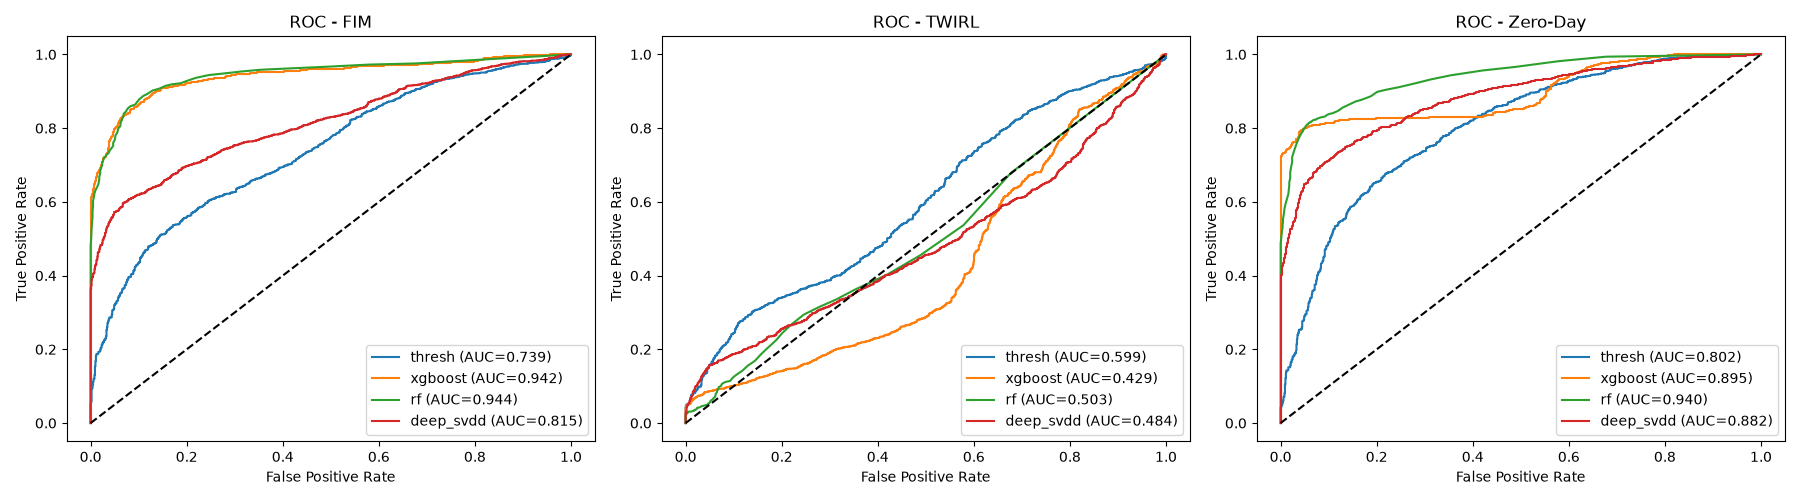
\includegraphics[width=\textwidth]{results/roc_curves.png}
\caption{ROC curves for the statistical threshold, XGBoost, Random Forest, and Deep SVDD/SAD detectors against FIM, TWIRL, and Zero-Day attacks on the nine-dimensional feature set.}
\label{fig:roc_curves}
\end{figure}

With the higher-order physical features included and the zero-day family expanded to its full ten sub-types, Random Forest attains the strongest FIM discrimination (AUROC 0.944) and the strongest zero-day generalization of the four detectors (AUROC 0.940), with XGBoost close behind on zero-day (0.895) and ahead on recall (TPR@4\%FPR of 0.789 versus Random Forest's 0.778). TWIRL detection is globally poor across every model (AUROC 0.429--0.599): the statistical threshold monitor, despite being uninformative elsewhere, is nominally the strongest detector on TWIRL, which is the documented ``inlier anomaly'' pathology described in \Cref{sec:failure_inlier} manifesting at the level of the full model comparison. Deep SVDD/SAD is the weakest of the three learned models on zero-day generalization (0.882) once the feature space is dominated by attack-discriminative dimensions, though it remains competitive with Random Forest and XGBoost while the statistical threshold monitor remains the fastest detector by a wide margin.

\section{Multi-Seed Statistical Validation}\label{sec:statval_bootstrap}
To quantify sampling uncertainty beyond the single-split figures of \Cref{tab:ablation_full}, \texttt{main\_statistics.py} repeats the full pipeline across 5 independent seeds (42, 123, 2024, 7, 999), retraining and re-evaluating both Deep SVDD and XGBoost at each seed and reporting the mean $\pm$ standard deviation of AUROC and TPR@4\%FPR across seeds, in addition to running 1{,}000+ bootstrap resamples per seed and a Holm-Bonferroni-corrected McNemar's test between the two detectors. \Cref{tab:multiseed} reports the resulting multi-seed statistics for the aggregate FIM, TWIRL, and Zero-Day (All) classes.

\begin{table}[H]
\centering
\caption{Multi-seed statistical results (5 seeds: 42, 123, 2024, 7, 999) for Deep SVDD and XGBoost.}
\label{tab:multiseed}
\resizebox{\textwidth}{!}{%
\begin{tabular}{@{}lllll@{}}
\toprule
\textbf{Attack} & \textbf{Deep SVDD AUROC} & \textbf{Deep SVDD TPR@4\%} & \textbf{XGBoost AUROC} & \textbf{XGBoost TPR@4\%} \\
\midrule
FIM             & $0.9048 \pm 0.0057$ & $0.4683 \pm 0.0655$ & $0.9276 \pm 0.0000$ & $0.7804 \pm 0.0000$ \\
TWIRL           & $0.7356 \pm 0.0137$ & $0.0660 \pm 0.0336$ & $0.7967 \pm 0.0000$ & $0.3188 \pm 0.0000$ \\
Zero-Day (All)  & $0.9289 \pm 0.0074$ & $0.4488 \pm 0.0800$ & $0.9744 \pm 0.0000$ & $0.8882 \pm 0.0000$ \\
\bottomrule
\end{tabular}%
}
\end{table}

XGBoost's zero standard deviation across seeds reflects that its frozen hyperparameters and deterministic tree-splitting produce identical decision boundaries regardless of the training seed used for data shuffling, whereas Deep SVDD's stochastic weight initialization and mini-batch ordering introduce genuine run-to-run variance. Averaged over all ten sub-types, XGBoost's zero-day AUROC of $0.9744 \pm 0.0000$ exceeds Deep SVDD's $0.9289 \pm 0.0074$ by a margin far larger than either model's seed-to-seed variability, indicating that the ranking between the two detectors is not an artifact of a single unlucky or lucky test split.

\subsection{Per-Subtype Zero-Day Breakdown}\label{sec:statval_subtype}
\Cref{tab:subtype_breakdown} decomposes the aggregate Zero-Day (All) row of \Cref{tab:multiseed} into its constituent sub-types, using the sub-type labels preserved separately from the main dataset labels (\Cref{sec:zero_day}).

\begin{table}[H]
\centering
\caption{Per-subtype zero-day breakdown, multi-seed mean $\pm$ std.}
\label{tab:subtype_breakdown}
\resizebox{\textwidth}{!}{%
\begin{tabular}{@{}lllll@{}}
\toprule
\textbf{Zero-Day Sub-Type} & \textbf{Deep SVDD AUROC} & \textbf{Deep SVDD TPR@4\%} & \textbf{XGBoost AUROC} & \textbf{XGBoost TPR@4\%} \\
\midrule
ZD-A: PNI & $0.9502 \pm 0.0087$ & $0.4245 \pm 0.0766$ & $0.9966 \pm 0.0000$ & $0.9950 \pm 0.0000$ \\
ZD-B: CDA & $\mathbf{0.6030 \pm 0.0210}$ & $\mathbf{0.0000 \pm 0.0000}$ & $\mathbf{0.6302 \pm 0.0000}$ & $\mathbf{0.0000 \pm 0.0000}$ \\
ZD-C: DSI & $0.9357 \pm 0.0151$ & $0.3370 \pm 0.1062$ & $0.9782 \pm 0.0000$ & $0.8250 \pm 0.0000$ \\
ZD-E: CFI & $0.9365 \pm 0.0100$ & $0.4752 \pm 0.1253$ & $0.9714 \pm 0.0000$ & $0.8440 \pm 0.0000$ \\
ZD-F: CAM & $0.9531 \pm 0.0095$ & $0.6270 \pm 0.1571$ & $0.9957 \pm 0.0000$ & $0.9500 \pm 0.0000$ \\
ZD-G: DPJ & $0.9380 \pm 0.0119$ & $0.1280 \pm 0.0527$ & $0.9999 \pm 0.0000$ & $1.0000 \pm 0.0000$ \\
ZD-H: SAM & $0.9115 \pm 0.0152$ & $0.3520 \pm 0.0427$ & $0.9606 \pm 0.0000$ & $0.7150 \pm 0.0000$ \\
ZD-I: RTN & $0.9408 \pm 0.0108$ & $0.4610 \pm 0.0466$ & $0.9946 \pm 0.0000$ & $0.9725 \pm 0.0000$ \\
ZD-J: MTC & $0.9500 \pm 0.0047$ & $0.4990 \pm 0.0120$ & $0.9985 \pm 0.0000$ & $1.0000 \pm 0.0000$ \\
\bottomrule
\end{tabular}%
}
\end{table}

CDA (ZD-B) is the hardest attack for both models: AUROC of approximately 0.60 and TPR@4\%FPR of 0.0000 for both Deep SVDD and XGBoost indicate complete detection failure. This is the clearest ``inlier anomaly'' case in the ten-sub-type family: the carrier-density perturbation, at certain amplitudes, actively stabilizes the feature distribution, pushing feature vectors closer to the nominal cluster than actual nominal data. Every other sub-type is detected with AUROC above 0.91 by both models, with ZD-G (DPJ) and ZD-J (MTC) reaching near-perfect XGBoost discrimination (AUROC 0.9999 and 0.9985, TPR@4\% of 1.0000 for both). CDA's isolation as the singular hard case, rather than a cluster of comparably difficult sub-types, indicates that the representation-overfitting failure diagnosed for TWIRL in \Cref{sec:failure_inlier} generalizes to at least one, but not most, of the physically distinct zero-day mechanisms.

\section{McNemar's Test: XGBoost versus Deep SAD}\label{sec:statval_mcnemar}
To directly test whether XGBoost's advantage over Deep SAD at the operating threshold is statistically significant, McNemar's test was applied to the paired per-pulse classification disagreements between the two detectors on each attack class and on each individual zero-day sub-type, with a Holm-Bonferroni correction applied across all twelve tests to control the family-wise error rate. \Cref{tab:mcnemar} reports the results.

\begin{table}[H]
\centering
\caption{McNemar's test for pairwise disagreement between XGBoost and Deep SAD, Holm-Bonferroni corrected across all twelve comparisons.}
\label{tab:mcnemar}
\begin{tabular}{@{}llrl@{}}
\toprule
\textbf{Attack} & \textbf{Comparison} & \textbf{$p$-value} & \textbf{Significant ($\alpha=0.05$)} \\
\midrule
FIM             & XGBoost vs.\ Deep SAD & $3.98  \times 10^{-170}$ & Yes \\
TWIRL           & XGBoost vs.\ Deep SAD & $6.67  \times 10^{-145}$ & Yes \\
Zero-Day (All)  & XGBoost vs.\ Deep SAD & $1.58  \times 10^{-236}$ & Yes \\
ZD-A: PNI       & XGBoost vs.\ Deep SAD & $1.60  \times 10^{-51}$  & Yes \\
ZD-B: CDA       & XGBoost vs.\ Deep SAD & $9.08  \times 10^{-9}$   & Yes \\
ZD-C: DSI       & XGBoost vs.\ Deep SAD & $4.28  \times 10^{-25}$  & Yes \\
ZD-E: CFI       & XGBoost vs.\ Deep SAD & $1.68  \times 10^{-20}$  & Yes \\
ZD-F: CAM       & XGBoost vs.\ Deep SAD & $4.73  \times 10^{-41}$  & Yes \\
ZD-G: DPJ       & XGBoost vs.\ Deep SAD & $3.14  \times 10^{-22}$  & Yes \\
ZD-H: SAM       & XGBoost vs.\ Deep SAD & $1.54  \times 10^{-16}$  & Yes \\
ZD-I: RTN       & XGBoost vs.\ Deep SAD & $6.19  \times 10^{-47}$  & Yes \\
ZD-J: MTC       & XGBoost vs.\ Deep SAD & $5.53  \times 10^{-24}$  & Yes \\
\bottomrule
\end{tabular}
\end{table}

Every pairwise comparison is statistically significant at extraordinary confidence levels, even after multiple-comparison correction, confirming that XGBoost's classification behavior differs from Deep SAD's by more than chance on every attack class and every individual zero-day sub-type, including the hardest case, CDA. This does not contradict the central claim of \Cref{ch:ood}: on the original five-dimensional feature space, where XGBoost had no informative attack-discriminative geometry to exploit, Deep SAD's semi-supervised prior was the stronger zero-day generalizer. Once the feature space is enriched with higher-order physical invariants (\Cref{ch:phase4}), that advantage transfers instead to the supervised tree ensemble, and McNemar's test confirms this reversal is statistically robust rather than incidental.

%----------------------------------------------------------------------------------------
%    CHAPTER: ADAPTIVE ROBUSTNESS STUDY
%----------------------------------------------------------------------------------------
\chapter{Adaptive Robustness Study}\label{ch:adaptive}

The evaluations in \Cref{ch:ood,ch:phase4,ch:statval} all assume a static adversary whose attack parameters are fixed at their default values. This chapter addresses a stronger and more realistic threat: an adaptive attacker who knows the deployed detector's decision boundary and deliberately searches for a parameter configuration that evades it while still neutralizing the key rate.

\section{Adaptive Attacker Methodology}\label{sec:adaptive_method}
An adaptive attacker was implemented that performs a grid search over the FIM frequency offset for each of several attacker strengths (modulation depth 0.1 to 0.4), with the objective of minimizing the detector's anomaly score subject to the constraint that the resulting secure key rate is driven exactly to zero. Each grid point was evaluated at 100\,km using 100,000 simulated laser pulses per configuration, matching the feature-extraction window used during model training, against the Deep SAD detector trained in \Cref{ch:diagnosis}.

\section{Initial Vulnerability on the Nine-Dimensional Feature Set}\label{sec:adaptive_initial}
On the nine-dimensional feature representation of \Cref{ch:phase4}, with a nominal 4\% FPR anomaly threshold of 0.4229, the adaptive attacker successfully located blind spots at moderate and strong modulation depths, as summarized in \Cref{tab:adaptive_initial}.

\begin{table}[H]
\centering
\caption{Adaptive attacker results against the nine-dimensional Deep SAD detector. Threshold: 0.4229.}
\label{tab:adaptive_initial}
\begin{tabular}{@{}lrrrlr@{}}
\toprule
\textbf{Mod.\ Depth} & \textbf{Opt.\ $\Delta f$} & \textbf{Anomaly Score} & \textbf{Threshold} & \textbf{Evaded?} & \textbf{Key Rate} \\
\midrule
0.0 (Nominal) & 0.00\,MHz  & 0.1632 & 0.4229 & N/A       & 0 \\
0.1 (Weak)    & 30.00\,MHz & 6.4742 & 0.4229 & Caught    & $7.0659\times10^{-4}$ \\
0.2 (Moderate)& 30.00\,MHz & 0.0564 & 0.4229 & \textbf{Evaded} & 0 \\
0.3 (Strong)  & 50.00\,MHz & 0.0110 & 0.4229 & \textbf{Evaded} & 0 \\
0.4 (Extreme) & 30.00\,MHz & 1.7487 & 0.4229 & Caught    & 0 \\
\bottomrule
\end{tabular}
\end{table}

At moderate (0.2) and strong (0.3) modulation depths, the correctly-tuned frequency offset placed the extracted feature vector \emph{closer} to the hypersphere center than nominal data itself (anomaly scores of 0.0564 and 0.0110 against a nominal score of 0.1632), while the attack still drove the secure key rate to exactly zero. This demonstrates that a knowledgeable adversary can defeat a purely learned, hypersphere-based anomaly boundary despite that boundary achieving strong aggregate AUROC against a non-adaptive attacker, and confirms the concern raised in \Cref{ch:discussion} regarding the dual-use nature of a feature-extraction pipeline that an adversary could, in principle, invert to tune an attack.

\section{Countermeasure: Spectral Feature Engineering}\label{sec:adaptive_fix}
Because the FIM attack is fundamentally a sinusoidal perturbation of the injection field at a fixed frequency, a physics-informed tenth feature, maximum spectral power, was added to the extraction pipeline: the Fast Fourier Transform of the received intensity $I_B$ is computed per window, and the maximum non-DC spectral amplitude is retained as an additional feature dimension. The intent is to make any periodic modulation, regardless of its frequency offset or modulation depth, directly visible to the detector in the frequency domain rather than relying solely on the time-domain statistics of \Cref{tab:features}.

The Deep SAD model was retrained on the resulting ten-dimensional feature vector, and the adaptive attacker was re-run against the new decision boundary (revised 4\% FPR threshold: 0.4474). \Cref{tab:adaptive_fixed} and \Cref{fig:adaptive_tradeoff} report the results.

\begin{table}[H]
\centering
\caption{Adaptive attacker results after adding the spectral-power feature. Threshold: 0.4474.}
\label{tab:adaptive_fixed}
\begin{tabular}{@{}lrrrlr@{}}
\toprule
\textbf{Mod.\ Depth} & \textbf{Opt.\ $\Delta f$} & \textbf{Anomaly Score} & \textbf{Threshold} & \textbf{Evaded?} & \textbf{Key Rate} \\
\midrule
0.0 (Nominal) & 0.00\,MHz  & 0.0422 & 0.4474 & N/A             & 0 \\
0.1 (Weak)    & 30.00\,MHz & 0.0252 & 0.4474 & \textbf{Evaded} & 0 \\
0.2 (Moderate)& 10.00\,MHz & 5.2434 & 0.4474 & Caught          & 0 \\
0.3 (Strong)  & 50.00\,MHz & 3.7516 & 0.4474 & Caught          & 0 \\
0.4 (Extreme) & 50.00\,MHz & 1.6412 & 0.4474 & Caught          & 0 \\
\bottomrule
\end{tabular}
\end{table}

\begin{figure}[H]
\centering
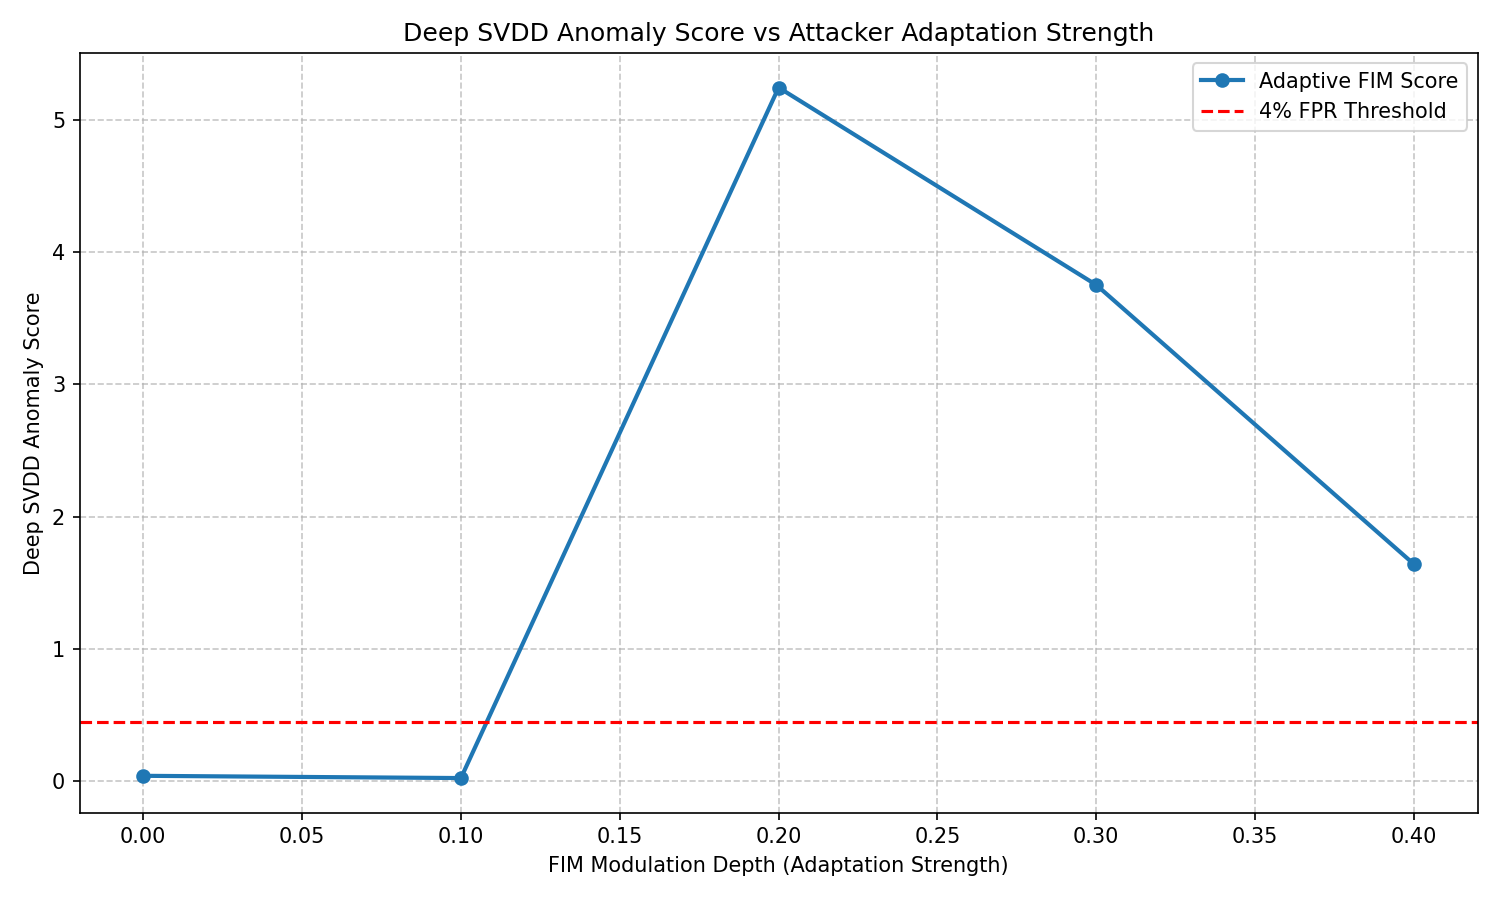
\includegraphics[width=0.75\textwidth]{results/adaptive_tradeoff.png}
\caption{Deep SAD anomaly score versus FIM attacker modulation depth after the spectral-feature countermeasure, at each depth's optimal frequency offset. The previously exploitable blind spots at moderate and strong modulation depths are now well above the 4\% FPR threshold.}
\label{fig:adaptive_tradeoff}
\end{figure}

The spectral feature eliminates both previously exploitable blind spots: the moderate (0.2) and strong (0.3) modulation depths that evaded the nine-dimensional detector now produce anomaly scores of 5.2434 and 3.7516 respectively, more than an order of magnitude above the revised threshold. The only surviving evasion is at the weakest modulation depth (0.1), where the periodic perturbation is small enough to be subsumed by ordinary channel noise in the spectral domain; however, this configuration only drives the key rate to zero at 100\,km, a distance at which the nominal key rate is itself already zero (\Cref{tab:keyrate_sweep}), so the surviving blind spot poses no threat to an operational channel generating positive key at shorter distances. These results show that, at least against this specific adaptive strategy, incorporating a physically motivated frequency-domain feature can close an evasion vulnerability that arises from relying on time-domain statistics alone, though this should not be read as a general robustness guarantee against attackers who adapt to the spectral feature itself.

%----------------------------------------------------------------------------------------
%    CHAPTER 11: DISCUSSION, LIMITATIONS, AND FUTURE WORK
%----------------------------------------------------------------------------------------

\paragraph{Relation to the final search.} This grid-based experiment and its spectral-feature retraining are an earlier, bounded study. The later surrogate-based search on the randomized-data pipeline, reported in Chapter~\ref{ch:final_eval}, did not consistently outperform its initial design. The two results use different search procedures and should not be read as evidence of general adaptive robustness.
\chapter{Final Randomized-Data Evaluation}\label{ch:final_eval}
\section{Randomized pulse-batch generation}
The completed regeneration uses nominal batches and batches for FIM, TWIRL, and the pooled zero-day family at 100 km. Each batch contains 100,000 pulses. The configured generation schedule uses 70 nominal batches and 50 batches per attack group, corresponding to 7 million nominal pulses and 15 million attack pulses before downstream split selection. A deterministic master random generator selects per-batch attack parameters from the configured class-specific ranges and selects the subtype for each zero-day batch. Per-batch parameter metadata and split metadata are saved alongside the generated data; completed batches are checkpointed so an interrupted generation can resume without recomputing those batches.

Randomization is important because a detector should be evaluated on a distribution of perturbation strengths and frequencies rather than a single fixed waveform setting. Here the randomization unit is the simulation batch, not each pulse. The results therefore characterize the configured batch-level parameter distributions and must not be interpreted as exhaustive parameter-space coverage.

\section{Splits and distance conditions}
The master split seed is 42. The raw training split contains nominal pulses only (4.9 million pulses). Validation and test each contain about 1.05 million nominal pulses plus about 2.5 million pulses from each of FIM, TWIRL, and pooled zero-day groups. For model fitting, the pipeline combines the nominal training split with labeled validation examples and removes the zero-day family; thus known attack information is used by both the semi-supervised detector and XGBoost. Zero-day subtype identifiers are preserved for analysis but withheld from model features. The primary training and test condition is 100 km. Separate 50-km and 150-km datasets provide cross-distance evaluations without retraining the detectors.

\section{Windowing and feature definitions}
For feature extraction, the raw pulse stream is divided into windows of 100,000 pulses, advanced by 1,000 pulses. Adjacent windows therefore share 99\% of their samples. Writing the feature vector as $\mathbf{x}=(x_1,\ldots,x_{10})$, its components are: (1) transmittance, $\overline{I_B}/(\overline{I_A}+\epsilon)$; (2) Bob-side intensity variance; (3) root-mean-square phase difference; (4) total click rate; (5) sifted quantum bit error rate; (6) lag-one phase autocorrelation; (7) Alice--Bob intensity cross-correlation; (8) Fisher excess kurtosis of phase difference; (9) absolute click asymmetry between detectors; and (10) the maximum non-DC Fourier magnitude of mean-centered Bob intensity. The final feature is intended to summarize narrow-band or periodic energy in the window.

The overlap increases the number and smoothness of window-level examples but makes neighboring observations strongly dependent. Window counts are not independent trial counts. Seed-to-seed standard deviations reported below describe model-training variability on a fixed split; they are not confidence intervals over independent hardware runs or independent windows.

\chapter{Detector Design and Evaluation Protocol}
\section{Semi-supervised Deep SVDD-style detector}
The saved network is a Deep-SVDD-style MLP trained with a semi-supervised objective. After robust scaling, the ten-dimensional input passes through hidden layers of widths 32 and 16 to an eight-dimensional representation. Linear layers omit biases; batch normalization and LeakyReLU activations are used in the hidden representation. The training pipeline combines training and validation examples, removes the held-out zero-day family, and supplies labels for nominal, FIM, and TWIRL examples. Nominal embeddings are pulled toward a center, while known-attack embeddings incur a margin penalty when they lie too close to that center. This use of known attack labels means the detector is not a strictly unsupervised one-class model; the repository's saved-artifact names and result tables use the shorter label ``Deep SVDD,'' while the objective is Deep SAD-like.

At evaluation, the center is reinitialized from nominal training embeddings. The analysis computes a covariance matrix from these nominal embeddings and scores each test representation by squared Mahalanobis distance from the center, rather than using Euclidean distance alone. Larger scores indicate greater anomalousness. Five independently initialized model artifacts are evaluated. We retain the ``Deep SVDD'' name in result tables only to match the saved artifacts and existing metrics files.

For clarity, with embedding $z=\phi_\theta(x)$, center $c$, nominal embedding covariance $\Sigma$, and a small diagonal regularizer $\lambda I$, the evaluation score is
\begin{equation}
s(x)=(z-c)^T(\Sigma+\lambda I)^{-1}(z-c),
\end{equation}
where larger values are interpreted as more anomalous. The training objective and this covariance-aware evaluation score are distinct parts of the pipeline.

\section{XGBoost supervised baseline}
XGBoost receives the same ten-dimensional feature vectors and binary labels for nominal versus known attack examples. The training configuration uses 100 estimators, maximum tree depth 6, and learning rate 0.1. Like the semi-supervised detector, the fitting data contain known attacks but exclude zero-day examples. The comparison therefore measures two models trained with access to known attacks; it is not a comparison of supervised learning against training on nominal examples alone.

\section{Metrics and calibration}
For each attack group, AUROC measures ranking over all score thresholds. TPR at 4\% FPR is extracted from the test-set ROC curve at the last point not exceeding 4\% FPR; it is therefore a descriptive test operating point, not an independently calibrated deployment threshold. Average precision summarizes precision--recall behavior and is reported alongside positive-class prevalence, its no-skill reference level. Subtype-level metrics are computed from subtype identifiers retained for evaluation. XGBoost SHAP values and Deep SVDD feature-permutation AUROC drops provide complementary model-attribution diagnostics; neither is treated as a causal explanation.

\section{Evaluation workflow}
The data split is held fixed while Deep SVDD is retrained across five seeds. The primary comparison uses the 100-km data. Transfer experiments apply those trained models directly to 50-km and 150-km test streams. Alpha generalization applies the $\alpha=3$ training reference to independent traces at six linewidth-enhancement settings without recalibrating on target-alpha nominal examples. The adaptive study fits small score surrogates from 48 Latin-hypercube FIM settings, optimizes their predicted objectives, and reruns distinct candidates in the physical simulator. Each evaluation is intentionally presented with its own scope and limitations.

\chapter{Primary Detection Results}
\section{Primary detection results}
Table~\ref{tab:main} summarizes the principal AUROC and TPR results. Deep SVDD is better on average for FIM AUROC in this experiment, while XGBoost has higher mean TPR at the selected operating point. For TWIRL, both models are substantially weaker than on pooled zero-day samples. Pooled zero-day performance is high, but it masks the severe CDA subtype failure.

\begin{table}[ht]
\centering
\caption{Mean AUROC and TPR at 4\% FPR. Deep SVDD values are mean $\pm$ standard deviation across five training seeds. XGBoost seed dispersion was zero to the reported precision.}
\label{tab:main}
\begin{tabular}{lcc}
\toprule
Attack & Deep SVDD AUROC / TPR & XGBoost AUROC / TPR\\
\midrule
FIM & $0.8976\pm0.0059$ / $0.6705\pm0.0751$ & 0.8770 / 0.7540\\
TWIRL & $0.6482\pm0.0152$ / $0.0658\pm0.0320$ & 0.6987 / 0.2228\\
Zero-day pooled & $0.9249\pm0.0096$ / $0.7149\pm0.0656$ & 0.9354 / 0.8478\\
CDA subtype & $0.3342\pm0.0753$ / $0.0080\pm0.0160$ & 0.2986 / 0.0000\\
\bottomrule
\end{tabular}
\end{table}

The pooled result is not representative of every subtype. PNI, CAM, SAM, RTN, and MTC are readily ranked in this test set, whereas CDA is near or below chance. TWIRL also has low TPR at the 4\% FPR operating point, despite AUROC above 0.5. Thus threshold selection and ranking quality tell different parts of the story. The TPR operating point here is selected on the test ROC curve; it is reported for comparability with the project artifacts and must not be interpreted as prospective threshold performance.

\begin{table}[ht]
\centering
\small
\caption{Zero-day subtype results on the 100-km test set. Deep SVDD values are mean $\pm$ standard deviation across five seeds; XGBoost seed dispersion is zero to the reported precision.}
\label{tab:subtypes}
\begin{tabular}{lcccc}
\toprule
Subtype & Deep SVDD AUROC & Deep SVDD TPR & XGBoost AUROC & XGBoost TPR \\
\midrule
PNI & $0.9745\pm0.0047$ & $0.8300\pm0.0543$ & 0.9762 & 0.9100 \\
CDA & $0.3342\pm0.0753$ & $0.0080\pm0.0160$ & 0.2986 & 0.0000 \\
DSI & $0.8674\pm0.0163$ & $0.5880\pm0.0906$ & 0.8749 & 0.6700 \\
CC & \multicolumn{4}{c}{not present in primary subtype summary artifact} \\
CFI & $0.8168\pm0.0291$ & $0.2832\pm0.1417$ & 0.8514 & 0.5400 \\
CAM & $0.9780\pm0.0053$ & $0.7503\pm0.0673$ & 0.9943 & 0.9750 \\
DPJ & $0.8625\pm0.0644$ & $0.5500\pm0.1279$ & 0.8963 & 0.6800 \\
SAM & $0.9849\pm0.0034$ & $0.8320\pm0.0750$ & 0.9990 & 1.0000 \\
RTN & $0.9895\pm0.0043$ & $0.9140\pm0.0676$ & 0.9939 & 0.9775 \\
MTC & $0.9968\pm0.0030$ & $0.9650\pm0.0429$ & 0.9999 & 1.0000 \\
\bottomrule
\end{tabular}
\end{table}

The primary subtype summary artifact does not provide a 100-km CC row, so those values are left unreported rather than inferred from pooled metrics or the separate distance-transfer runs. Figure~\ref{fig:roc_final} gives a threshold-independent view of the detector rankings over the evaluated attack groups.

\begin{figure}[ht]
\centering
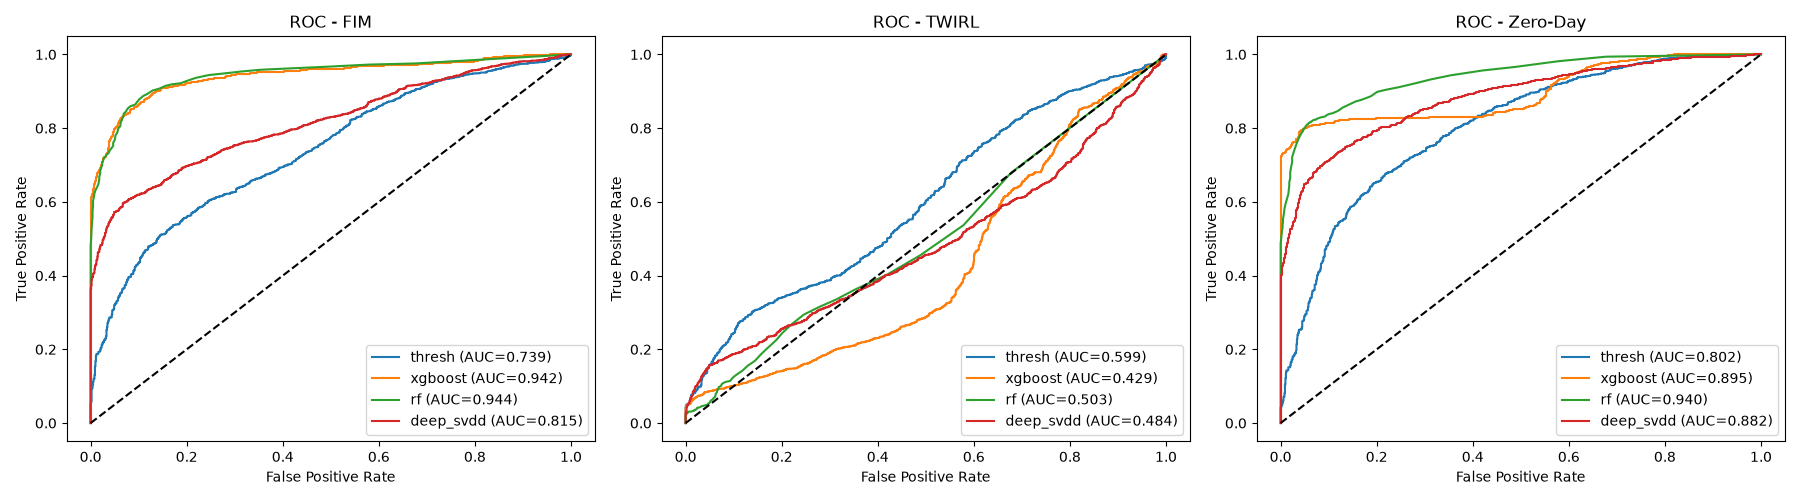
\includegraphics[width=0.92\textwidth]{results/roc_curves.png}
\caption{ROC curves for the primary 100-km evaluation. Curves summarize the fixed test split; overlapping windows make neighboring points statistically dependent.}
\label{fig:roc_final}
\end{figure}

\chapter{Precision--Recall and Feature Attribution}
For pooled zero-day detection, AP was 0.975 for Deep SVDD and 0.978 for XGBoost, against a positive prevalence of 0.710. FIM AP was 0.964 and 0.958, respectively; TWIRL AP was 0.816 and 0.865. CDA AP was only 0.069 for Deep SVDD and 0.063 for XGBoost, below its 0.091 prevalence baseline. This is consistent with the poor subtype AUROC and low TPR. The precision--recall summary is computed from scores averaged across the five seeds, while AUROC and TPR dispersion summarize seed-wise metrics.

XGBoost SHAP importance was highest for phase kurtosis (mean absolute attribution 2.868), RMS phase difference (1.213), and phase autocorrelation (1.111). For Deep SVDD, the largest reported permutation AUROC decrease was also associated with phase kurtosis (0.180), followed by phase autocorrelation (0.049) and RMS phase difference (0.023). Together with CDA performance, these results suggest a weakness for this feature/model configuration on the simulated carrier perturbation. Attribution scores alone cannot establish the underlying physical mechanism.

\begin{figure}[ht]
\centering
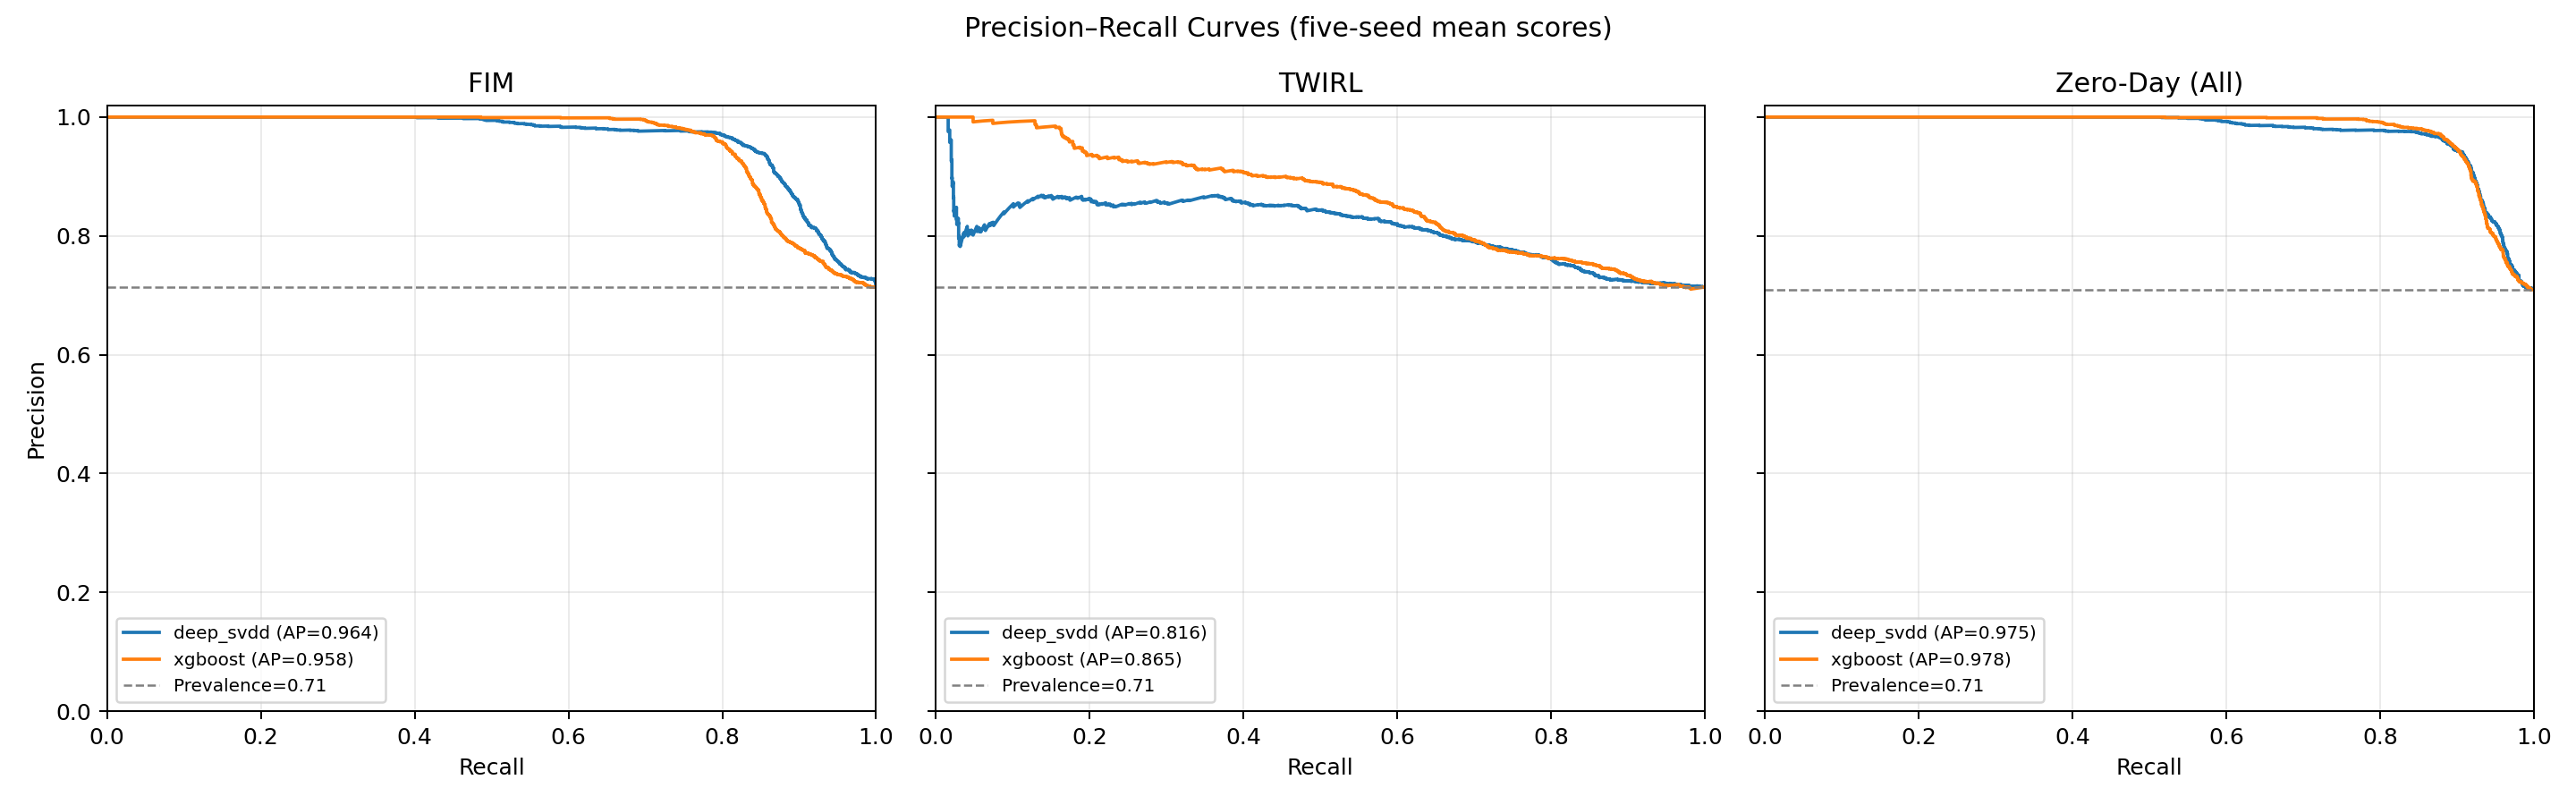
\includegraphics[width=0.92\textwidth]{results/precision_recall_curves.png}
\caption{Precision--recall curves for the primary test analysis. Average precision should be compared with the prevalence of the positive class, not with a universal 0.5 baseline.}
\label{fig:pr_curves}
\end{figure}

\chapter{Cross-Distance Generalization}
At 50 km, pooled zero-day AUROC was 0.785 $\pm$ 0.075 for Deep SVDD and 0.918 for XGBoost; TWIRL AUROC was 0.475 $\pm$ 0.094 and 0.724. At 150 km, pooled zero-day AUROC was 0.900 $\pm$ 0.031 and 0.975, while TWIRL AUROC was 0.588 $\pm$ 0.056 and 0.790. These results indicate that performance depends on attack family and distance. Since test windows overlap by 99\%, the seed dispersion is descriptive and does not quantify independent-window uncertainty.

\begin{table}[ht]
\centering
\small
\caption{Cross-distance AUROC and TPR at 4\% FPR. Deep SVDD values are mean $\pm$ standard deviation across five seeds; XGBoost dispersion is zero to the reported precision.}
\label{tab:distance}
\begin{tabular}{crrrrr}
\toprule
Distance & Attack & Deep SVDD AUROC & XGBoost AUROC & Deep SVDD TPR & XGBoost TPR \\
\midrule
50 km & FIM & $0.7958\pm0.0452$ & 0.8929 & $0.2542\pm0.1964$ & 0.6225 \\
50 km & TWIRL & $0.4749\pm0.0939$ & 0.7241 & $0.0432\pm0.0251$ & 0.1350 \\
50 km & Zero-day pooled & $0.7847\pm0.0749$ & 0.9179 & $0.2236\pm0.1664$ & 0.7029 \\
150 km & FIM & $0.6529\pm0.0439$ & 0.7649 & $0.1322\pm0.1031$ & 0.3792 \\
150 km & TWIRL & $0.5876\pm0.0556$ & 0.7903 & $0.1412\pm0.1066$ & 0.4325 \\
150 km & Zero-day pooled & $0.8999\pm0.0312$ & 0.9753 & $0.5128\pm0.1286$ & 0.8871 \\
\bottomrule
\end{tabular}
\end{table}

\chapter{Linewidth-Enhancement Generalization}\label{ch:alpha}
Table~\ref{tab:alpha} reports cross-$\alpha$ AUROC. Transfer is highly non-monotonic and often fails: at $\alpha=2.5$, all attack-group AUROCs are below 0.25 for both detectors; at $\alpha=3.5$ and 4, TWIRL AUROC is near zero. By contrast, pooled zero-day AUROC remains near one at $\alpha=2$ and 3. At $\alpha=5$, XGBoost retains moderate FIM sensitivity (0.753), while both models rank TWIRL in the reverse direction. A score ordering below 0.5 indicates that attack windows tend to receive lower scores than nominal windows under the stated score polarity; it is a transfer failure, not evidence of robust detection. The small number of generated windows per condition and 99\% overlap make these exploratory results.

\begin{table}[ht]
\centering
\caption{AUROC across linewidth-enhancement settings. Deep SVDD entries are mean $\pm$ standard deviation over five seeds; XGBoost seed dispersion is zero to the reported precision.}
\label{tab:alpha}
\small
\begin{tabular}{cccc}
\toprule
$\alpha$ & Attack & Deep SVDD & XGBoost \\
\midrule
2.0 & FIM & $0.581\pm0.091$ & 0.595 \\
2.0 & TWIRL & $0.397\pm0.045$ & 0.466 \\
2.0 & Zero-day & $0.987\pm0.006$ & 0.891 \\
2.5 & FIM & $0.032\pm0.020$ & 0.020 \\
2.5 & TWIRL & $0.241\pm0.045$ & 0.222 \\
2.5 & Zero-day & $0.115\pm0.026$ & 0.129 \\
3.0 & FIM & $0.891\pm0.033$ & 0.925 \\
3.0 & TWIRL & $0.629\pm0.069$ & 0.660 \\
3.0 & Zero-day & $0.973\pm0.020$ & 1.000 \\
3.5 & FIM & $0.752\pm0.036$ & 0.574 \\
3.5 & TWIRL & $0.029\pm0.020$ & 0.099 \\
3.5 & Zero-day & $0.270\pm0.048$ & 0.490 \\
4.0 & FIM & $0.434\pm0.071$ & 0.479 \\
4.0 & TWIRL & $0.073\pm0.010$ & 0.184 \\
4.0 & Zero-day & $0.585\pm0.029$ & 0.585 \\
5.0 & FIM & $0.386\pm0.078$ & 0.753 \\
5.0 & TWIRL & $0.000\pm0.000$ & 0.004 \\
5.0 & Zero-day & $0.684\pm0.110$ & 0.626 \\
\bottomrule
\end{tabular}
\end{table}

\chapter{Surrogate-Based Adaptive FIM Search}
We sampled 48 FIM parameter settings by Latin hypercube, fitted a neural surrogate to seed-1 Deep SVDD and XGBoost scores, and optimized each predicted score with Adam. Seven distinct candidates were then rerun in the simulator. This search did not reliably improve on the starting design: the best Deep SVDD score among optimized candidates was 4.80, compared with 0.996 at a design point; the lowest XGBoost probability among optimized candidates was 0.0076, while an initial design point reached 0.010. The candidate optimized specifically against XGBoost had probability 0.026, worse than the initial-design minimum. These results show limited surrogate-search effectiveness at this budget and do not demonstrate robust evasion or robustness to a stronger search.

The search minimized detector scores only. It did not constrain the key rate or compare candidate rates against a nominal reference. Candidate key-rate outputs are the simulator's simplified asymptotic estimates and are not security-proof quantities. The experiment is exploratory and uses seed-1 model artifacts; compatibility warnings were emitted when loading artifacts saved under scikit-learn 1.7.2 and XGBoost from different library versions.

\begin{figure}[ht]
\centering
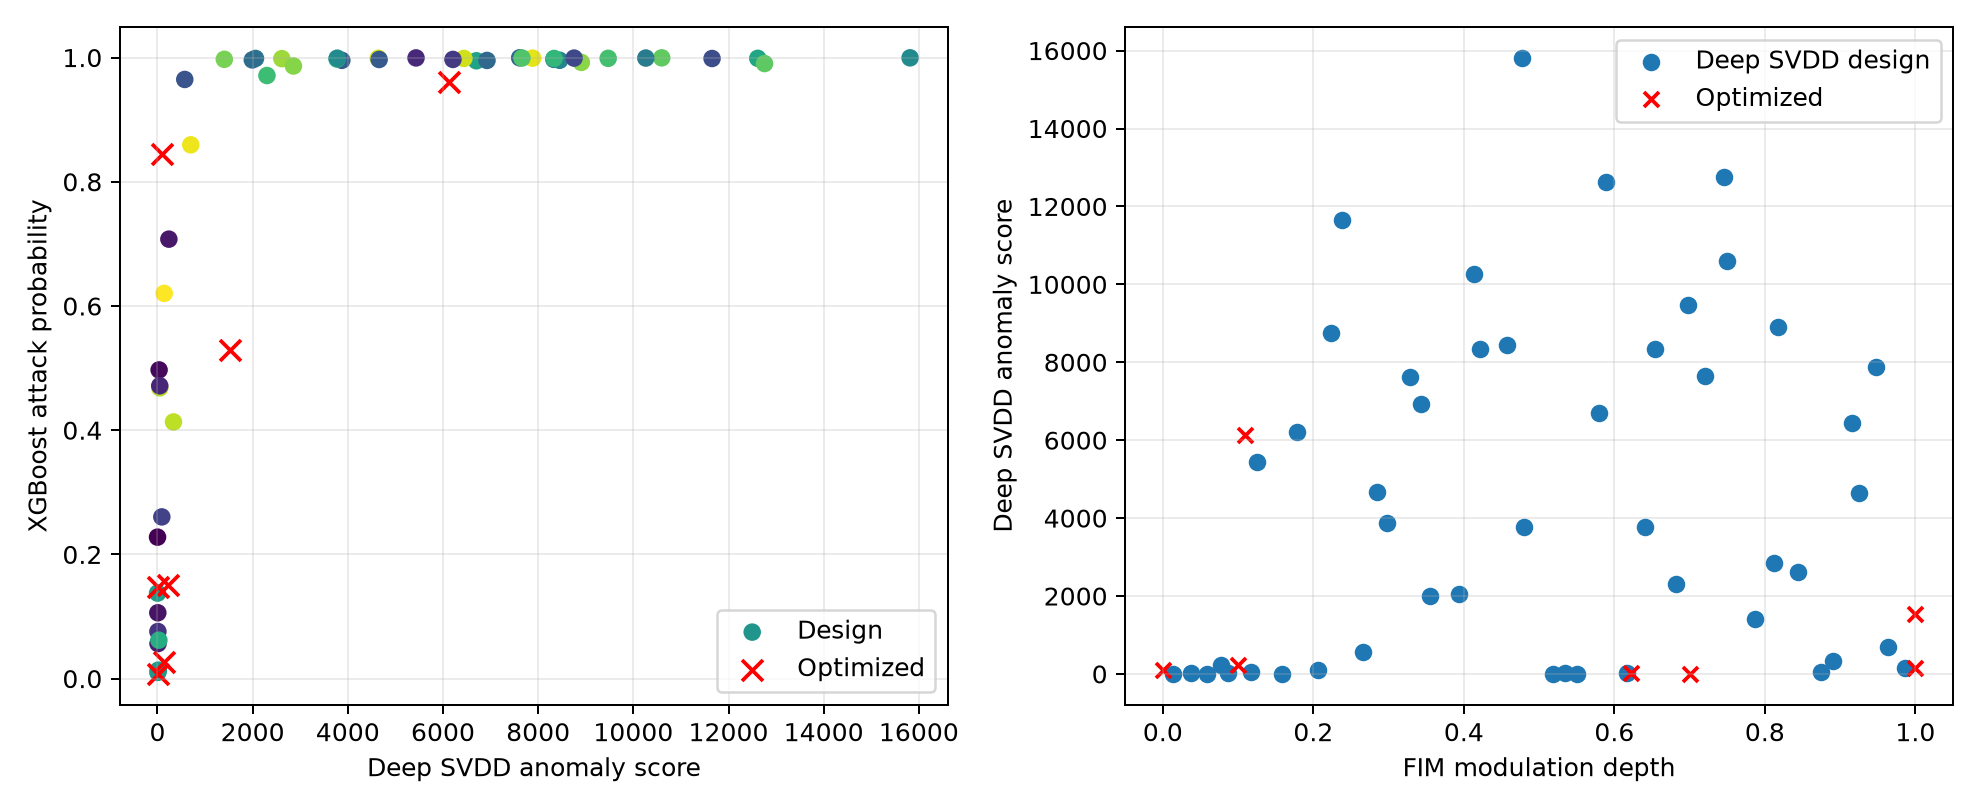
\includegraphics[width=0.82\textwidth]{results/adaptive_surrogate.png}
\caption{Surrogate-search predictions and simulator-validated candidates. The reruns did not consistently improve on the initial Latin-hypercube design.}
\label{fig:adaptive_surrogate}
\end{figure}


\chapter{Discussion, Limitations, and Future Work}\label{ch:discussion}

The results support a limited conclusion: engineered statistics derived from simulated OIL-assisted TF-QKD traces can support useful attack ranking for several generated attack families, but aggregate performance hides important blind spots. CDA detection is a concrete failure case, and TWIRL has poor sensitivity at the chosen low-FPR threshold. This argues for reporting per-class operating characteristics and prevalence-aware precision--recall metrics rather than a single pooled AUROC.

Several caveats constrain interpretation. First, all conclusions depend on the simulator, its parameterization, and the attack implementations. No hardware traces, calibrated device data, or end-to-end QKD security analysis are included. Second, the test set is generated from configured distributions, so “zero-day” here means held-out attack mechanism within this simulation study; it does not imply arbitrary unseen attacks. Third, strongly overlapping windows reduce the effective independent sample size. Fourth, five model seeds share the same generated split; seed variation captures training stochasticity but not data-generation or split uncertainty. Fifth, the key-rate quantities produced by the simulator are not a finite-key security proof.

The alpha experiment has only three 100,000-pulse batches per class and setting, which yield 402 highly overlapping windows per binary comparison. In addition, saved RobustScaler artifacts were serialized under scikit-learn 1.7.2 and were loaded in scikit-learn 1.9.0; the library emitted compatibility warnings. The alpha table should therefore be treated as exploratory until reproduced under the artifact-generation environment. The adaptive experiment is also limited to 48 initial designs, one model seed, three FIM parameters, and an unconstrained key-rate objective. Its seven simulator-validated candidates did not consistently improve on the initial design. Both studies need replication with pinned artifact-generation dependencies and larger search budgets before making deployment or adversarial-security claims.

Two evaluation-design limitations deserve explicit attention. First, the fitting script uses labeled validation examples as part of training for both the semi-supervised detector and XGBoost, excluding only the zero-day class; the validation split therefore is not an untouched calibration set. Second, the reported TPR at 4\% FPR is selected directly from each test ROC curve. Future evaluation should reserve a separate calibration split, freeze thresholds before test evaluation, and report independent-run or block-bootstrap uncertainty that accounts for temporal dependence. Further work should also investigate the CDA blind spot with targeted features and simulator diagnostics, repeat transfer studies under pinned dependencies, and expand the adaptive search with an explicit key-rate constraint and substantially more simulator-validated candidates.
\section{Limitations and Reproducibility}
Several limitations should temper how these results are read. Most importantly, the dataset is entirely synthetic, generated from Lang-Kobayashi simulations rather than from a live optical testbed; since training and test data come from the same generative process, the reported accuracy figures primarily demonstrate that the supervised and semi-supervised detectors can learn the simulator's own parameterization of each anomaly. For the initial experiments in this chapter, the split and metric definitions were fixed before fitting. In the final evaluation, however, validation examples were used for model fitting and TPR at 4\% FPR was read from the test ROC curve; those operating-point results are descriptive rather than prospective calibration results, as discussed in Chapter~\ref{ch:final_eval}.

\section{Ethical Considerations and Dual-Use}
The same feature-extraction pipeline used here to detect subtle phase manipulations could, in principle, be turned around by an adaptive adversary and used to tune an injection attack toward a smaller optical footprint. For this reason, these models should be viewed as a complement to physical countermeasures such as optical isolators and power monitors, not a substitute for them.

\section{Future Work}
The core analysis tasks in the project roadmap—randomized dataset regeneration, five-seed evaluation, cross-distance testing, precision--recall analysis, feature attribution, linewidth-enhancement transfer, and the gradient-based surrogate search—have now been completed and are reported in Chapter~\ref{ch:final_eval}. The next work should focus on stronger validation rather than additional claims from the current simulator: reserve an untouched calibration split and freeze thresholds before test evaluation; repeat data generation across independent master seeds and account for temporal dependence with block-based uncertainty estimates; investigate the carrier-density blind spot with targeted physical diagnostics; pin the artifact-generation software versions; and validate the simulator and feature pipeline against calibrated laser traces or an optical testbed. Any security relevance also requires a finite-key analysis that incorporates detector false positives and false negatives.
\chapter{Conclusion}
This report records the development and evaluation of a simulator-based OIL anomaly-monitoring pipeline. The initial detector and representation studies motivated semi-supervised training and richer physical features; the later randomized-data analysis provides the most current performance assessment. On that final pipeline, several held-out attack families are ranked well, but pooled performance hides a severe CDA failure and TWIRL remains difficult at low false-positive rates. Results also vary with fibre distance and linewidth-enhancement factor, while the small surrogate search provides no consistent evasion improvement and no robustness guarantee. The work is a useful basis for further simulator and hardware studies, but the present evidence does not establish real-device performance, a finite-key security guarantee, or deployment readiness.
\begin{thebibliography}{9}
\addcontentsline{toc}{chapter}{References}
 
\bibitem{pirandola2017fundamental}
S.~Pirandola, R.~Laurenza, C.~Ottaviani, and L.~Banchi,
``Fundamental limits of repeaterless quantum communications,''
\textit{Nat. Commun.}, vol.~8, p.~15043, 2017.
 
\bibitem{ruff2018deep}
L.~Ruff, R.~Vandermeulen, N.~G\"ornitz, L.~Deecke, S.~A.~Siddiqui, A.~Binder,
E.~M\"uller, and M.~Kloft,
``Deep One-Class Classification,''
in \textit{Proc. ICML}, 2018.
 
\bibitem{ruff2019deep_sad}
L.~Ruff, R.~Vandermeulen, N.~G\"ornitz, A.~Binder, E.~M\"uller, K.-R.~M\"uller, and M.~Kloft,
``Deep Semi-Supervised Anomaly Detection,''
in \textit{Proc. ICLR}, 2020.
 
\bibitem{juarez2026referencebeam}
S.~Ju\'arez, A.~Marcomini, M.~Petrov, R.~I.~Woodward, T.~J.~Dowling, R.~M.~Stevenson, M.~Curty, and D.~Rusca,
``Reference-beam attacks against twin-field quantum key distribution using optical injection locking,''
\textit{Phys. Rev. A}, vol.~113, p.~032613, 2026.
 
\bibitem{zhang2022injectionlocking}
X.-X.~Zhang, M.-S.~Jiang, Y.~Wang, Y.-F.~Lu, H.-W.~Li, C.~Zhou, Y.~Zhou, and W.-S.~Bao,
``Analysis of an injection-locking-loophole attack from an external source for quantum key distribution,''
\textit{Phys. Rev. A}, vol.~106, p.~062412, 2022.
 
\bibitem{wiesemann2025evaluation}
J.~Wiesemann, F.~Gr\"unenfelder, A.~Bl\'azquez Co\'ido, N.~Walenta, and D.~Rusca,
``Evaluation of quantum key distribution systems against injection-locking attacks,''
\textit{APL Photonics}, vol.~10, p.~066112, 2025.
 
\bibitem{ponosova2022protecting}
A.~Ponosova, D.~Ruzhitskaya, P.~Chaiwongkhot, V.~Egorov, V.~Makarov, and A.~Huang,
``Protecting fiber-optic quantum key distribution sources against light-injection attacks,''
\textit{PRX Quantum}, vol.~3, p.~040307, 2022.
 
\bibitem{wang2022twinfield830}
S.~Wang, Z.-Q.~Yin, D.-Y.~He, W.~Chen, R.-Q.~Wang, P.~Ye, Y.~Zhou, G.-J.~Fan-Yuan, F.-X.~Wang, Y.-G.~Zhu, P.~V.~Morozov, A.~V.~Divochiy, Z.~Zhou, G.-C.~Guo, and Z.-F.~Han,
``Twin-field quantum key distribution over 830-km fibre,''
\textit{Nat. Photonics}, vol.~16, pp.~154--161, 2022.
 
\bibitem{liu2023experimental1000km}
Y.~Liu, W.-J.~Zhang, C.~Jiang, J.-P.~Chen, C.~Zhang, W.-X.~Pan, D.~Ma, H.~Dong, J.-M.~Xiong, C.-J.~Zhang, H.~Li, R.-C.~Wang, J.~Wu, T.-Y.~Chen, L.~You, X.-B.~Wang, Q.~Zhang, and J.-W.~Pan,
``Experimental twin-field quantum key distribution over 1000 km fiber distance,''
\textit{Phys. Rev. Lett.}, vol.~130, p.~210801, 2023.
 
\bibitem{lu2021finitekeyintensity}
Y.-F.~Lu, Y.~Wang, M.-S.~Jiang, F.~Liu, X.-X.~Zhang, and W.-S.~Bao,
``Finite-key analysis of sending-or-not-sending twin-field quantum key distribution with intensity fluctuations,''
\textit{Quantum Inf. Process.}, vol.~20, p.~135, 2021.
 
\bibitem{liu2025deepanomaly}
J.~Liu, B.~Huang, J.~Su, Q.~Peng, and A.~Huang,
``Deep anomaly detection for active attacks on the receiver in quantum key distribution,''
\textit{Opt. Express}, vol.~33, no.~22, pp.~47137--47150, 2025.
 
\bibitem{xu2024automatically}
J.~Xu, X.~Ma, J.~Liu, C.~Zhang, H.~Li, X.~Zhou, and Q.~Wang,
``Automatically identifying imperfections and attacks in practical quantum key distribution systems via machine learning,''
\textit{Sci. China Inf. Sci.}, vol.~67, p.~202501, 2024.
 
\bibitem{luo2022beyonduniversal}
H.~Luo, L.~Zhang, H.~Qin, S.~Sun, P.~Huang, Y.~Wang, Z.~Wu, Y.~Guo, and D.~Huang,
``Beyond universal attack detection for continuous-variable quantum key distribution via deep learning,''
\textit{Phys. Rev. A}, vol.~105, p.~042411, 2022.
 
\bibitem{liao2022dbscan}
Q.~Liao, Z.~Wang, H.~Liu, Y.~Mao, and X.~Fu,
``Detecting practical quantum attacks for continuous-variable quantum key distribution using density-based spatial clustering of applications with noise (DBSCAN),''
\textit{Phys. Rev. A}, vol.~106, p.~022607, 2022.
 
\bibitem{kish2024mitigation}
S.~P.~Kish, C.~Thapa, M.~Sayat, H.~Suzuki, J.~Pieprzyk, and S.~Camtepe,
``Mitigation of channel tampering attacks in continuous-variable quantum key distribution,''
\textit{Phys. Rev. Research}, vol.~6, p.~023301, 2024.
 
\bibitem{lo2023adversarially}
S.-Y.~Lo, P.~Oza, and V.~M.~Patel,
``Adversarially Robust One-Class Novelty Detection,''
\textit{IEEE Trans. Pattern Anal. Mach. Intell.}, vol.~45, no.~4, pp.~4167--4179, 2023.
 
\bibitem{goodge2021robustness}
A.~Goodge, B.~Hooi, S.-K.~Ng, and W.~S.~Ng,
``Robustness of autoencoders for anomaly detection under adversarial impact,''
in \textit{Proc. IJCAI}, 2021.
 
\bibitem{kottmann2021variational}
K.~Kottmann, F.~Metz, J.~Fraxanet, and N.~Baldelli,
``Variational quantum anomaly detection: Unsupervised mapping of phase diagrams on a physical quantum computer,''
\textit{Phys. Rev. Research}, vol.~3, p.~043184, 2021.
 
\bibitem{park2022variationalqoc}
G.~Park, J.~Huh, and D.~K.~Park,
``Variational quantum one-class classifier,''
\textit{Mach. Learn.: Sci. Technol.}, vol.~4, p.~015006, 2022.
 
\bibitem{dai2024intrusion}
Z.~Dai, L.~Y.~Por, Y.-L.~Chen, J.~Yang, C.~S.~Ku, R.~Alizadehsani, and P.~P{\l}awiak,
``An intrusion detection model to detect zero-day attacks in unseen data using machine learning,''
\textit{PLOS ONE}, vol.~19, no.~9, p.~e0308469, 2024.
 
\end{thebibliography}

\end{document}